\section{Matrix estimation for generalized block models}
\label{sec:W}

%
In this section we phrase a result essentially due to Abbe and Sandon \cite{DBLP:conf/nips/AbbeS16} (and closely related to results by Bordenave et al \cite{DBLP:conf/focs/BordenaveLM15}) in somewhat more general terms.
This turns out to be enough to capture an algorithm to estimate a pairwise-vertex-similarity matrix in the $d,k,\alpha,\e$ mixed-membership block model when $\e^2 d > k^2 (\alpha+1)^2$.

Let $\cU$ be a universe of labels, endowed with some base measure $\nu$, such that $\int 1 \cdot d\nu = 1$.
Let $\mu$ be a probability distribution on $\cU$, with a density relative to $\nu$.
(We abuse notation by conflating $\mu$ and its associated density).
Let $W\colon \cU \times \cU \rightarrow \R_+$ be a bounded nonnegative function with $W(x,y) = W(y,x)$ for every $x,y \in \cU$.
Consider a random graph model $G(n,d,W,\mu)$ sampled as follows.
For each of $n$ vertices, draw a label $x_i \sim \mu$ independently.
Then for each pair $ij \in [n]^2$, independently add the edge $(i,j)$ to the graph with probability $\tfrac dn W(x_i,x_j)$.
(This captures the $W$-random graph models used in literature on graphons.)

Let $\cF$ denote the space of square-integrable functions $f \colon \cU \rightarrow \R$, endowed with the inner product $\iprod{f,g} = \E_{x \sim \mu} f(x) g(x)$.
That is, $f \in \cF$ if $\E_{x \sim \mu} f(x)^2$ exists.

We assume throughout that
\begin{enumerate}
  \item (Stochasticity) For every $x \in \cU$, the average $\E_{y \sim \mu} W(x,y) = 1$.
  \item (Finite rank) $W$ has a finite-rank decomposition $W(x,y) = \sum_{i \leq r} \lambda_i f_i(x) f_i(y)$ where $\lambda_i \in \R$ and $f_i \colon \cU \rightarrow \R$.
  The values $\lambda_i$ are the eigenvalues of $W$ with respect to the inner product generated by $\mu$.
  The eigenfunctions are orthonormal with respect to the $\mu$ inner product.
  Notice that the assumptions on $W$ imply that its top eigenfunction $f_1(x)$ is the constant function, with eigenvalue $\lambda_1 = 1$.
  \item (Niceness I) Certain rational moments of $\mu^{-1}$ exist; that is $\E_{x \sim \mu} \mu(x)^{-t}$ exists for $t = -3/2, -2$.
  \item (Niceness II) $W$ and $\mu$ are nice enough that $W(x,y) \leq 1/ \sqrt{\mu(x) \mu(y)}$ and $|\overline{W}(x,y)| \leq \lambda_2 / \sqrt{\mu(x) \mu(y)}$ for every $x,y \in \cU$, where $\overline{W}(x,y) = W(x,y) - 1$.
  (Notice that in the case of discrete $W$ and $\mu$ this is always true, and for smooth enough $W$ and $\mu$ it is true via a $\delta$-function argument.)
\end{enumerate}
The function $W$ induces a Markov operator $W \colon \cF \rightarrow \cF$.
If $f \in \cF$, then
\[
  (W f) (x) = \E_{y \sim \mu} W(x,y) f(y)\mper
\]
(We abuse notation by conflating the function $W$ and the Markov operator $W$.)
%


\begin{theorem}[Implicit in \cite{DBLP:conf/nips/AbbeS16}]
\label{thm:W-main}
  Suppose the operator $W$ has eigenvalues $1 = \lambda_1 > \lambda_2 > \dots > \lambda_r$ (each possibly with higher multiplicity) and $\delta \defeq 1 - \tfrac 1 {d \lambda_2^2} > 0$.
  Let $\Pi$ be the projector to the second eigenspace of the operator $W$.
  For types $x_1,\ldots,x_n \sim \mu$, let $A \in \R^{n \times n}$ be the random matrix $A_{ij} = \Pi(x_i,x_j)$, where we abuse notation and think of $\Pi \colon \cU \times \cU \rightarrow \R$.
  There is an algorithm with running time $n^{\poly(1/\delta)}$ which outputs an $n \times n$ matrix $P$ such that for $x,G \sim G(n,d,W,\mu)$,
  \[
  \E_{x,G} \Tr P \cdot A \geq \delta^{O(1)} \cdot (\E_{x,G} \|A\|^2)^{1/2} (\E_{x,G} \|P\|^2)^{1/2}\mper
  \]
\end{theorem}

When $\cU$ is discrete with $k$ elements one recovers the usual $k$-community stochastic block model, and the condition $\lambda_2^2 > 1$ matches the Kesten-Stigum condition in that setting.
When $\lambda_2^2 > 1 + \delta$, the guarantees of Abbe and Sandon can be obtained by applying the above theorem to obtain an estimator $P$ for the matrix $M = \sum_{s \in [k]} v_s v_s^\top$, where $v_s$ is the centered indicator vector of community $s$.
The estimator $P$ will have at least $\delta^{O(1)}/k$ correlation with $M$, and a random vector in the span of the top $k/\delta^{O(1)}$ eigenvectors of $M$ will have correlation $(\delta/k)^{O(1)}$ with some $v_s$.
Thresholding that vector leads to the guarantees of Abbe and Sandon for the $k$-community block model, with one difference: Abbe and Sandon's algorithm runs in $O(n \log n)$ time, much faster than the $n^{\poly(1/\delta)}$ running time outlined above.
In essence, they achieve this by computing an estimator $P'$ for $M$ which counts only non-backtracking paths in $G$ (the estimator $P$ counts \emph{self-avoiding} paths).

In Section~\ref{sec:mm-matrix-main} we prove a corollary of Theorem~\ref{thm:W-main}.
This yields the algorithm discussed Theorem~\ref{thm:mm-intro-matrix} for the mixed-membership blockmodel.
As discussed before, the quantitative recovery guarantees of this algorithm are weaker than those of our final algorithm, whose recovery accuracy depends only on the distance $\delta$ of the signal-to-noise ratio of the mixed-membership blockmodel to $1$.
In Section~\ref{sec:W-main-proof} we prove Theorem~\ref{thm:W-main}.

\subsection{Matrix estimation for the mixed-membership model}
\label{sec:mm-matrix-main}
We turn to the mixed-membership model and show that Theorem~\ref{thm:W-main} yields an algorithm for partial recovery in the mixed-membership block model.
However, the correlation of the vectors output by this algorithm with the underlying community memberships depends both on the signal-to-noise ratio and the number $k$ of communiteis.
(In particular, when $k$ is super-constant this algorithm no longer solves the partial recovery task.)

\begin{definition}[Mixed-Membership Block Model]
Let $G(n, d, \epsilon, \alpha, k)$ be the following random graph ensemble.
For each node $i \in [n]$, sample a probability vector $\sigma_i \in \R^k_{\geq 0}$ with $\sum_{t \in [k]} \sigma_i(t) = 1$ according to the following (simplified) Dirichlet distribution.
\[
\Pr(\sigma) \propto \prod_{t \in [k]} \sigma_i(t)^{\alpha/k - 1}
\]
For each pair of vertices $i,i' \in [n]$, sample communities $t \sim \sigma_i$ and $t' \sim \sigma_{i'}$.
  If $t = t'$, add the edge $\{ i,i' \}$ to $G$ with probability $\tfrac d n (1 + (1 - \tfrac 1 k) \epsilon)$.
  If $t \neq t'$, add the edge $\{ i,i' \}$ to $G$ with probability $\tfrac d n (1 - \tfrac \epsilon k)$.
(For simplicity, throughout this paper we consider only the case that the communities have equal sizes and the connectivity matrix has just two unique entries.)
\end{definition}

\begin{theorem}[Constant-degree partial recovery for mixed-membership block model, $k$-dependent error]\torestate{\label{thm:mm-main-warmup}
For every $\delta > 0$ and $d(n),\e(n),k(n),\alpha(n)$, there is an algorithm with running time $n^{O(1) + 1/\delta^{O(1)} }$ with the following guarantees when
  \[
  \delta \defeq 1 - \frac{k^2(\alpha +1)^2}{\e^2 d} > 0 \quad \text{ and } \quad k,\alpha  \le n^{o(1)} \text{ and } \epsilon^2 d \le n^{o(1)} \mper
  \]
Let $\sigma, G \sim G(n,d,\epsilon,k,\alpha)$ and for $s \in [k]$ let $v_s \in \R^n$ be given by $v_s(i) = \sigma_i(s) - \tfrac 1 k$.

   The algorithm outputs a vector $x$ such that $\E \iprod{x,v_1}^2 \geq \delta' \|x\|^2 \|v_1\|^2$, for some $\delta' \geq (\delta/k)^{O(1)}$.\footnote{The requirement $\epsilon^2 d \leq n^{o(1)}$ is for technical convenience only; as $\epsilon^2 d$ increases the recovery problem only becomes easier.}}
\end{theorem}

Ideally one would prefer an algorithm which outputs $\tau_1,\ldots,\tau_n \in \Delta_{k-1}$ with $\corr(\sigma,\tau) \geq \delta'/(\alpha+1)$.
If one knew that $\iprod{x,v_1} \geq \delta' \|x\| \|v\|$ rather than merely the guarantee on $\iprod{x,v_1}^2$ (which does not include a guarantee on the sign of $x$), then this could be accomplished by correlation-preserving projection, Theorem~\ref{thm:correlation-preserving-projection}.
The tensor methods we use in our final algorithm for the mixed-membership model are able to obtain a guarantee on $\iprod{x,v_1}$ and hence can output probability vectors $\tau_1,\ldots,\tau_n$.\footnote{Such a guarantee could be obtained here by using a cross-validation scheme on $x$ to choose between $x$ and $-x$. Since we are focused on what can be accomplished by matrix estimation methods generally we leave this to the reader.}

To prove Theorem~\ref{thm:mm-main-warmup} we will apply Theorem~\ref{thm:W-main} and then a simple spectral rounding algorithm; the next two lemmas capture these two steps.
\begin{lemma}[Mixed-membership block model, matrix estimation]\label{lem:mm-W-conditions}
  If $\cU$ is the $(k-1)$-simplex, $\mu$ is the $\alpha,k$ Dirichlet distribution, and $W(\sigma,\sigma') = 1 - \tfrac \e k + \e \iprod{\sigma,\sigma'}$, then $G(n,d,W,\mu)$ is the mixed-membership block model with parameters $k,d,\alpha,\e$.
  In this case, the second eigenvalue of $W$ has multiplicity $k-1$ and has value $\lambda_2 = \tfrac{\e}{k(\alpha +1)}$.
\end{lemma}
\begin{proof}
  The first part of the claim follows from the definitions.
  For the second part, note that $W$ has the following decomposition
  \[
  W(\sigma,\tau) = 1 + \sum_{i \leq k} \e (\sigma_i - \tfrac 1k) (\tau_i - \tfrac 1k)\mper
  \]
  The functions $\sigma \mapsto \sigma_i - \tfrac 1k$ are all orthogonal to the constant function $\sigma \mapsto 1$ with respect to $\mu$; i.e.
  \[
  \E_{\sigma \sim \mu} 1 \cdot (\sigma_i - \tfrac 1k) = 0
  \]
  because $\E \sigma_i = \tfrac 1k$.

  It will be enough to test the above Rayleigh quotient
  \[
    \frac{\E_{\sigma \sim \mu} f(\sigma) \cdot (Wf)(\sigma)}{\E_{\sigma \sim \mu} f(\sigma)^2}
  \]
  with any function $f(\sigma)$ in the span of the functions $\sigma \mapsto \sigma_i - \tfrac 1k$.
  If we pick $f(\sigma) = \sigma_1 - \tfrac 1k$ the remaining calculation is routine, using only the second moments of the Dirichlet distribution (see Fact~\ref{fact:dirichlet-covariance-warmup} below).
\end{proof}

\begin{fact}[Special case of Fact~\ref{fact:dirichlet-covariance}]
  \label{fact:dirichlet-covariance-warmup}
  Let $\sigma \in \R^k$ be distributed according to the $\alpha,k$ Dirichlet distribution.
  Let $\tsigma = \sigma - \tfrac 1k \cdot 1$ be centered.
  Then $\E (\tsigma)(\tsigma)^\top = \tfrac 1 {k(\alpha +1)} \cdot \Pi$ where $\Pi$ is the projector to the complement of the all-$1$s vector in $\R^k$.
\end{fact}

We analyze a simple rounding algorithm.
\begin{lemma}\label{lem:mm-warmup-rounding}
  Let $M = \sum_{i=1}^k v_i v_i^\top$ be an $n\times n$ symmetric rank-$k$ PSD matrix.
  Let $P \in \R^{n \times n}$ be another symmetric matrix such that $\iprod{P,M} \geq \delta \|P\| \|M\|$ (where $\| \cdot \|$ is the Frobenious norm).
  Then for at least one vector $v$ among $v_1,\ldots,v_k$, a random unit vector $x$ in the span of the top $(k/\delta)^{O(1)}$ eigenvectors of $P$ satisfies
  \[
    \E \iprod{x,v}^2 \geq (\delta/k)^{O(1)} \|v\|^2 \mper
  \]
\end{lemma}

Now we can prove Theorem~\ref{thm:mm-main-warmup}.
\begin{proof}[Proof of Theorem~\ref{thm:mm-main-warmup}]
  Lemma~\ref{lem:mm-W-conditions} shows that the conditions of Theorem~\ref{thm:W-main} hold, and hence (via color coding) there is an $n^{\poly(1/\delta)}$ time algorithm to compute a matrix $P$ such that $\iprod{P,M} \geq \delta^{O(1)} \|P\| \|M\|$ with probability at least $\delta^{O(1)}$, where $M = \sum_{s \in [k]} v_s v_s^\top$.
  (The reader may check that the matrix $A$ of Theorem~\ref{thm:W-main} is in this case the matrix $M$ described here.)

  Applying Lemma~\ref{lem:mm-warmup-rounding} shows that a random unit vector $x$ in the span of the top $(k/\delta)^{O(1)}$ eigenvectors of $P$ satisfies $\iprod{x,v}^2 \geq (\delta/k)^{O(1)} \|v\|^2$, where $v \in \R^n$ has entries $v_i = \sigma_i(1)$.
  (The choice of $1$ is without loss of generality.)
\end{proof}

\subsection{Proof of Theorem~\ref{thm:W-main}}
\label{sec:W-main-proof}
\begin{definition}
  For a pair of functions $A,B \colon \cU \times \cU \rightarrow \R$, we denote by $AB$ their product, whose entries are $(AB)(x,y) = \E_{z \sim \mu} A(x,z)B(z,y)$.
\end{definition}

The strategy to prove Theorem~\ref{thm:W-main} will as usual be to apply Lemma~\ref{lem:basis-conditions}.
We check the conditions of that Lemma in the following Lemmas, deferring their proofs till the end of this section.

\begin{lemma}\label{lem:W-unbiased}
  Let $G_{ij}$ be the $0/1$ indicator for the presence of edge $i \sim j$ in a graph $G$.
  As usual, let $\saw_\ell(i,j)$ be the collection of simple paths of length $\ell$ in the complete graph on $n$ vertices from $i$ to $j$.

  Let $x,G \sim G(n,d,W,\mu)$.
  Let $\alpha \in \saw_\ell(i,j)$.
  Let $p_\alpha(G) = \prod_{ab \in \alpha} (G_{ab} - \tfrac dn)$.
  Let $\overline{W}(x,y) = W(x,y) - 1$.
  Then
  \[
    \E\Brac{p_\alpha(G) \mid x_i, x_j} = \Paren{\frac dn}^{\ell} \overline{W}^{\ell -1}(x_i,x_j)
  \]
\end{lemma}
\begin{lemma}\label{lem:W-pairwise}
  With the same notation as in Lemma~\ref{lem:W-unbiased}, as long as $\ell \geq C \log n / \delta^{O(1)}$ for a large-enough constant $C$,
  \[
  \Paren{\frac nd}^{2\ell} \sum_{\alpha,\beta \in \saw_\ell(i,j)} \E p_\alpha(G) p_\beta(G) \leq \delta^{-O(1)} \cdot |\saw_\ell(i,j)|^2 \cdot \E \overline{W}^{\ell-1}(x_i,x_j)^2\mper
  \]
  (The constant $C$ depends on $W$ and the moments of $\mu$.)
\end{lemma}

\begin{proof}[Proof of Theorem~\ref{thm:W-main}]
  Let $B_{ij} = \lambda_2^{-(\ell -1)} \overline{W}^{\ell -1}(x_i,x_j)$.
  By Lemma~\ref{lem:W-unbiased}, Lemma~\ref{lem:W-pairwise}, and Lemma~\ref{lem:basis-conditions}, there is matrix polynomial $P(G)$, computable to $1/\poly(n)$-accuracy in time $n^{\poly(1/\delta)}$ by color coding, such that
  \[
    \E \Tr PB^T \geq \delta^{O(1)} (\E \|P\|^2)^{1/2} (\E \|B\|^2)^{1/2}\mper
  \]
  At the same time, $B - A$ has entries
  \[
  (B-A)_{ij} = \sum_{3 \leq t \leq r} \Paren{\frac{\lambda_t}{\lambda_2}}^{\ell -1} \Pi_t(x_i,x_j) 
  \]
  where the $\Pi_t$ projects to the $t$-th eigenspace of $W$.
  Since $W$ is bounded, choosing $\ell$ a large enough multiple of $\log n$ ensures that $\E \|B-A\|^2 \leq n^{-100} \E \|B\|^2$, so the theorem now follows by standard manipulations.
\end{proof}


\subsection{Proofs of Lemmas}
\begin{proof}[Proof of Lemma~\ref{lem:W-unbiased}]
  As usual, we simply expand $p$, obtaining
  \begin{align*}
    \E\Brac{p_\alpha(G) \mid x_i, x_j} & = \E_x\Brac{ \prod_{ab \in \alpha} \frac dn \cdot (W_{x_a,x_b} - 1) \mid x_i, x_j}\\
    & = \Paren{\frac dn}^{\ell} \cdot \overline{W}^{\ell-1}(x_i,x_j)\mper\qedhere
  \end{align*}
\end{proof}


We will need some small facts to help in proving Lemma~\ref{lem:W-pairwise}.
\newcommand{\oW}{\overline{W}}
\begin{fact}\label{fact:W-frob}
  If $\ell - t \geq C \log n$ for large enough $C = C(W)$, then
  \[
    \lambda_2^{2t} \E_{x,y \sim \mu} \oW^{\ell -t}(x,y)^2 \leq (1 + o(1)) \cdot \E_{x,y \sim \mu} \oW^{\ell}(x,y)^2\mper
  \]
  Also, for any $t \leq \ell$,
  \[
    \lambda_2^{2t} \E_{x,y \sim \mu} \oW^{\ell -t}(x,y)^2 \leq r \cdot \E_{x,y \sim \mu} \oW^{\ell}(x,y)^2\mper
  \]
  where $r$ is the rank of $W$.
\end{fact}
\begin{proof}
  Using the eigendecomposition of $\oW$, we have that $\E_{x,y \sim \mu} \oW^{\ell -t}(x,y)^2 = \sum_{2 \leq i \leq r} \lambda_i^{2(\ell -t)}$ and similarly $\E_{x,y \sim \mu} \oW^{\ell}(x,y)^2 = \sum_{2 \leq i \leq r} \lambda_i^{2\ell}$.
  If $i > 2$, then
  \[
  \lambda_2^{2t} \lambda_i^{2(\ell -t)} = \lambda_2^{2\ell} (\lambda_i / \lambda_2)^{2(\ell -t)} \leq \lambda_2^{2\ell}/n
  \]
  by our assumption that $\ell -t \geq C \log n$ for large enough $C$.
  This finishes the proof of the first claim; the second one is similar.
\end{proof}

\begin{proof}[Proof of Lemma~\ref{lem:W-pairwise}]
  Pairs $\alpha,\beta$ which share only the vertices $i,j$ each contribute exactly $\E \overline{W}^{\ell -1}(x_i,x_j)^2$ to the left-hand side, by Lemma~\ref{lem:W-unbiased}.
  Consider next the contribution of $\alpha,\beta$ whose shared edges form paths originating at $i$ and $j$.
  Suppose there are $t$ such shared edges.
  Then
  \begin{align*}
    \E p_\alpha p_\beta & = \Paren{\frac dn}^{2\ell - t} \E_x \prod_{ab\in \alpha \triangle \beta} \overline{W}(x_a,x_b) \cdot \prod_{ab \in \alpha \cap \beta} (W(x_a,x_b) + O(d/n))\\
    & = \Paren{\frac dn}^{2\ell -t} (1 + O(d/n))^t \E \overline{W}^{2(\ell -t -1)} (x,y)^2 \mcom
  \end{align*}
  where for the second equality we used the assumption $\E_{x \sim \mu} W(x,y) = 1$ for every $y$.

  If $\ell - t > C \log n$ for the constant in Fact~\ref{fact:W-frob}, then this is at most $(1 + o(1)) \Paren{\frac dn}^{2\ell-t} \lambda_2^{- 2t} \E \overline{W}^{2(\ell -1 )} (x,y)^2$, and for every $t \leq \ell$ it is at most $ r \cdot \Paren{\frac dn}^{2\ell-t} \lambda_2^{-2t} \E \overline{W}^{2(\ell -1 )} (x,y)^2$.

  There are at most $|\saw_\ell(i,j)|^2/n^t \cdot t$ choices for such pairs $\alpha,\beta$, except when $t = \ell$, in which case there are $|\saw_\ell(i,j)|^2 / n^{t-1}$ choices.
  So the total contribution from such $\alpha,\beta$ is at most
  \begin{align*}
    & |\saw_\ell(i,j)|^2 \cdot \E_{x,y} \overline{W}^{\ell-1}(x,y)^2 \cdot \Paren{ \sum_{t \leq \ell/2} t d^{-t}  \lambda_2^{-2t} + nr \cdot \sum_{\ell \geq t > \ell/2} t d^{-t} \lambda_2^{-2t} }\\
    & \leq \delta^{-O(1)} |\saw_\ell(i,j)|^2 \E_{x,y} \overline{W}^{\ell-1}(x,y)^2\mper
  \end{align*}

  It remains to handle pairs $\alpha,\beta$ which share $t$ vertices and $s$ edges for $t > s$.
  If $t,s \leq \ell -2$, then there are only $n^{2(\ell-1) - s} \ell^{O(t-s)}$ choices for such a pair $\alpha,\beta$.
  The contribution of each such pair we bound as follows
  \begin{align*}
  \E p_\alpha p_\beta & = \Paren{\frac dn}^{2\ell - s} \E \prod_{ab \in \alpha \cap \beta} \E(G_{ab} - \tfrac dn)^2 \cdot \prod_{ab \in \alpha \triangle \beta} \overline{W}_{x_a,x_b}\mper
  \end{align*}
  Now, $\E\Brac{ (G_{ab} - \tfrac dn)^2  \, | \, x} = \tfrac dn (W(x_a,x_b) + O(d/n))$ by straightforward calculations, so the above is
  \begin{align*}
      & (1 + O(d/n))^s \Paren{\frac dn}^{2\ell - s} \E_x \prod_{ab \in \alpha \cap \beta} W(x_a,x_b) \cdot \prod_{ab \in \alpha \triangle \beta} \overline{W}(x_a,x_b)\\
      & \leq (1 + O(d/n))^s \Paren{\frac dn}^{2\ell - s} \lambda_2^{2\ell - s} \prod_{a \in \alpha \cup \beta} \mu(x_a)^{-\deg_{\alpha,\beta}(a)/2}
  \end{align*}
  where $\deg_{\alpha,\beta}(a)$ is the degree of the vertex $a$ in the graph $\alpha \cup \beta$.
  Any degree-$2$ vertices simply contribute $1$ in the above, since $\E_{x \sim \mu} 1/\mu(x) = 1$.
  There are at most $t -s$ vertices of higher degree; they may have degree at most $4$.
  They each contribute at most some number $C = C(\mu)$ by the niceness assumptions on $\mu$.
  So the above is at most
  \[
  (1 + o(1)) \Paren{\frac dn}^{2\ell - s} \lambda_2^{2\ell -s} \exp \{ O(t-s) \}\mper
  \]
  Putting things together as in Lemma~\ref{lem:indep-sbm} finishes the proof.
\end{proof}

\begin{proof}[Proof of Lemma~\ref{lem:mm-warmup-rounding}]
  By averaging, there is some $v$ among $v_1,\ldots,v_k$ such that
  \[
  \iprod{P,vv^\top} \geq \frac \delta k \cdot \|P\| \cdot \|M\| \geq \frac \delta k \cdot \|P\| \cdot \|vv^\top\|
  \]
  where the second inequality uses $M \succeq 0$.
  Renormalizing, we may assume $\|P\|$ has Frobenious norm $1$ and $v$ is a unit vector; in this case we obtain $\iprod{v,Pv} \geq \delta/k$.
  Writing out the eigendecomposition of $P$, let $P = \sum_{i=1}^n \lambda_i u_i u_i^\top$ and we get
  \[
    \sum_{i=1}^n \lambda_i \iprod{v,u_i}^2 \geq \delta/k
  \]
  By Cauchy-Schwartz,
  \[
  \sum_{i=1}^n \lambda_i \iprod{v,u_i}^2 \leq \Paren{\sum_{i=1}^n \lambda_i^2 \iprod{v,u_i}^2}^{1/2}
  \]
  and hence $\sum_{i=1}^n \lambda_i^2 \iprod{v,u_i}^2 \geq (\delta/k)^2$, while $\sum_{i=1}^n \lambda_i^2 = 1$.
  Now the Lemma follows from Markov's inequality.
\end{proof}

\iffalse
\section{Warmup II: mixed-membership block model with few communities}
\Dnote{}
\label{sec:mm-warmup}
We turn to the mixed-membership community model.
In this section we show how to to easily adapt two-community block model the algorithm from the previous section to the mixed-membership setting.
The resulting algorithm achieves a partial recovery guarantee, albeit with error depending strongly on the number of communities.
The algorithm is suitable for the setting that the number of communities $k = O(1)$, and it is strong enough to capture as a special case the algorithm of Abbe and Sandon \cite{DBLP:conf/nips/AbbeS16} in the setting that the block model connectivity matrix has only two distinct entries $1 + \e$ and $1 - \e$.
\footnote{We believe that the present algorithms can also obtain the guarantees of Abbe and Sandon for the case of general connectivity matrices but we leave this to future work.}
In the next section we describe our final algorithm for the mixed-membership block model, showing how to remove this $k$-dependence by estimating tensors rather than matrices.


As promised, the algorithm in this case looks very similar to our version of the two-community block model algorithm, Algorithm~\ref{alg:sbm}.
The only difference is in the second step, where we skip the rounding phase used in the $2$-community algorithm to output a $\pm 1$-valued vector.
\begin{algorithm}
  \label{alg:mm-warmup}
  For a given $n$-vertex graph $G$ with average degree $d$ and parameters $\delta,k > 0$, execute the following steps:
 \begin{compactenum}
  \item  evaluate the following matrix-valued polynomial $P(x) = (P_{ij}(x))$,
  \[
    P_{ij}(x)
    \coloneq \tfrac 1 {\card{\saw_\ell(i,j)}}
    \sum_{\alpha\in \saw_\ell(i,j)} p_\alpha(x)\,.
  \]
  Here, $\saw_\ell(i,j) \subseteq \binom n 2 $ consists of all sets of vertex pairs that form a simple (self-avoiding) path between $i$ and $j$ of length $\ell=\Theta(\log n) / \delta^{O(1)}$.
  The polynomials $p_\alpha$ are as in Algorithm~\ref{alg:sbm}.
  \item output $k$ independent random unit vectors $x_1,\ldots,x_k$ in the span of the top $C$ eigenvectors of $P$, for appropriate $C = \poly(k/\delta)$.
  \footnote{To recover the guarantees of the $k$-communtiy algorithm of Abbe and Sandon \cite{DBLP:conf/nips/AbbeS16} in the special case that the community connectivity matrix has only entries $1 + \e$ and $1-\e$, one may apply the rounding phase of Algorithm~\ref{alg:sbm} instead.
  The analysis is straightforward by combining the present analysis of the first step of this algorithm with the analysis of the Gaussian threshold rounding from Section~\ref{sec:warmup}.}
  \end{compactenum}
\end{algorithm}

The analysis will parallel the analysis of Algorithm~\ref{alg:sbm} from Section~\ref{sec:warmup}.
The main difference is the polynomial $P$ is no longer an estimator for a rank-one matrix $yy^\top$ where $y$ is a $\pm 1$-valued vector of community labels.
Instead, the polynomial $P$ estimates the rank-$k$ matrix $M = \sum_{s \in [k]} v_s v_s^\top$, where $v_s \in \R^n$ has $i$-th entry $v_s(i) = \sigma_i(s) - \tfrac 1k$, where $\sigma_i(s)$ is the amount of probability mass the $i$-th vertex places in community $s$.

As before, to analyze the algorithm we use two main tools.
First we show that the polynomials $p_\alpha$ are unbiased approximately pairwise independent estimators of the entries of $M$.
Then we give a straightforward analysis of the spectral rounding step.
The following lemmas are proved in Section~\ref{sec:mm-warmup-estimator} and Section~\ref{sec:mm-warmup-deferred}, respectively.

\begin{lemma}\label{lem:mm-warmup-estimators}
  Let $\sigma_1,\ldots,\sigma_n$ be iid draws from the $\alpha,k$ Dirichlet distribution and let $x$ be a sample from the $\e,k$ mixed-membership block model with labels $\sigma_1,\ldots,\sigma_n$.
  Let $v_s$ and $M$ be as above, and $p_\alpha$ as in Algorithm~\ref{alg:mm-warmup}.

  Let $\delta \defeq 1 - \tfrac{k^2 (\alpha+1)^2}{\e^2 d}$.
  The polynomial $P(x)$ satisfies
  \[
    \E \iprod{P(x), M} \geq \delta^{O(1)} (\E \|P(x)\|^2)^{1/2} (\E \|M\|^2)^{1/2}\mper
  \]
\end{lemma}




\subsection{Low-degree estimate for posterior second moment}
\label{sec:mm-warmup-estimator}
Remember that if $x \in \{0,1\}^{[n]^2}$ is a graph, the polynomial $p_\alpha$ for $\alpha \subseteq [n]^2$ is a product of centered edge indicators: 
\[
  p_\alpha(x)= \prod_{ab \in \alpha} \Paren{x_{ab}-\tfrac dn}\mper
\]

As usual, to prove Lemma~\ref{lem:mm-warmup-estimators} we will just check the conditions of Lemma~\ref{lem:basis-conditions}, which requires that the polynomials $p_\alpha$ are unbiased and approximately pairwise independent estimators of the entries of $M$.
The first step is the following fact, a mild adaptation of Fact~\ref{fact:edge-sbm}.
The proof is a straightforward calculation; we defer it to Section~\ref{sec:mm-warmup-deferred}.
\begin{fact}
  \label{fact:Ge-given-sigma}
  Consider a pair $\{i,j\} \in {\binom{n}{2}}$.
  For a probability vector $\sigma \in \R^k$ let $\tsigma = \sigma - \tfrac 1 k \cdot 1$.
  For $\sigma,G \sim G(n,d,\epsilon, \alpha, k)$,
  \begin{align*}
    & \E[p_{ij} \mid \sigma_i, \sigma_{j}] =\frac dn \epsilon\iprod{\tsigma_i,\tsigma_j}\mper\\
    & \E[p_{ij}^2 \mid \sigma_i, \sigma_{j}] = \frac dn \Brac{1 + \e \iprod{\tsigma_i,\tsigma_j} + O(\tfrac dn)}\mper
  \end{align*}
\end{fact}

Now we can check the first condition of Lemma~\ref{lem:basis-conditions}.
\begin{fact}
  \label{fact:mm-warmup-unbiased}
  Let $\alpha \subseteq \binom{n}{2}$ be a self-avoiding path between $i$ and $j$ in $[n]$, of length $\ell$.
  For $\sigma,G \sim G(n,d,\epsilon, \alpha, k)$,
  \[
    \Paren{\frac {nk(\alpha +1)} {\e d}}^{\ell} \cdot \frac 1 {k(\alpha+1)} \cdot \E \Brac{p_\alpha \mid \sigma_i, \sigma_j} = \iprod{\tsigma_i, \tsigma_j}
  \]
\end{fact}
\begin{proof}
  Expanding $p_\alpha$, we obtain
  \begin{align*}
    \E_\sigma \E_x \Brac{ p_\alpha  \mid \sigma} & = \Paren{\frac dn \epsilon}^{\ell} \E_\sigma \prod_{ab \in \alpha} \iprod{\tsigma_a,\tsigma_b} \text{ by Fact~\ref{fact:Ge-given-sigma} and conditional independence of $p_{ab}$'s}\\
    & = \Paren{\frac dn \epsilon}^\ell \cdot \Paren{\frac 1 {k(\alpha+1)}}^{\ell-1} \iprod{\tsigma_i, \tsigma_j} \text{ by Fact~\ref{fact:dirichlet-covariance-warmup}}\mper\qedhere
  \end{align*}
\end{proof}

Finally, we can check the second, approximate pairwise independence condition of Lemma~\ref{lem:basis-conditions}.
The proof is a straightforward modification of the proof of Lemma~\ref{lem:indep-sbm} so we leave it to the reader.
\begin{fact}
  \label{fact:mm-warmup-low-variance}
  For $\e,d,k,\alpha$ as in Lemma~\ref{lem:mm-warmup-estimators}, let $\delta = 1 - \tfrac{k^2(\alpha+1)^2}{\e^2 d}$.
  If $\delta > 0$ and $\ell \geq C \log n / \delta^{O(1)}$ for a large enough constant $C$, then for every distinct $i,j \in [n]$,
  \[
    \E \iprod{\tsigma_i, \tsigma_j}^2 \cdot \E \sum_{\alpha,\beta \in \saw_\ell(i,j)} \E p_\alpha(x) p_\beta(x) \leq \delta^{-O(1)} \cdot \sum_{\alpha,\beta \in \saw_\ell(i,j)} (\E p_\alpha(x) \iprod{\tsigma_i, \tsigma_j}) \cdot (\E p_\beta(x) \iprod{\tsigma_i,\tsigma_j})\mper
  \]
\end{fact}



\subsection{Deferred proofs}
\label{sec:mm-warmup-deferred}
\begin{proof}[Proof of Fact~\ref{fact:Ge-given-sigma}]
  We prove the first statement; the second is similar.
  The proof is just by expanding and rearranging terms.
  Note that
  \begin{align*}
    \Pr \{ \{i,i'\} \text{ is an edge in $G$} \mid \sigma_i, \sigma_{i'} \} & = \iprod{\sigma_i, \sigma_{i'}} \cdot \tfrac d n (1 + (1 - \tfrac 1 k)\epsilon) + (1 - \iprod{\sigma_i, \sigma_{i'}}) \cdot \tfrac d n (1 - \tfrac \epsilon k)\\
    & = \tfrac d n \cdot \Brac{(1 - \tfrac \epsilon k) + \epsilon \iprod{\sigma_i, \sigma_{i'}}}\mper
  \end{align*}
  (As a sanity check, if $\iprod{\sigma_i, \sigma_{i'}} = 0$, which is to say that $i$ and $i'$ are never in the same community, then this is just $\tfrac d n \cdot (1 - \tfrac \epsilon k)$, exactly the probability an edge is present between two nodes in differing communities.)
  Thus,
  \[
    \E\Brac{p_{ij}(x) \mid \sigma_i, \sigma_j} = \frac dn \e (\iprod{\sigma_i,\sigma_j} - \frac 1k) = \frac dn \e \iprod{\tsigma_i, \tsigma_j}\mper\qedhere
  \]
\end{proof}
\fi

\section{Tensor estimation for mixed-membership block models}
\label{sec:mm}

\subsection{Main theorem and algorithm}


%

\begin{theorem}[Constant-degree partial recovery for mixed-membership block model]\label{thm:mm-main}
There is a constant $C$ such that the following holds.
Let $G(n,d,\e,k,\alpha)$ be the mixed-membership block model.
For every $\delta \in (0,1)$ and $d(n),\e(n),k(n),\alpha(n)$, there is an algorithm with running time $n^{O(1) + 1/\delta^{O(1)} }$ with the following guarantees when
  \[
  \delta \defeq 1 - \frac{k^2(\alpha +1)^2}{\e^2 d} > 0 \quad \text{ and } \quad k,\alpha  \le n^{o(1)} \text{ and } \epsilon^2 d \le n^{o(1)} \mper
  \]
Let $\sigma, G \sim G(n,d,\epsilon,k,\alpha)$.
Let $t = (\alpha+1) \cdot \tfrac k {k+\alpha}$ (samples from the $\alpha,k$ Dirichlet distribution are approximately uniform over $t$ coordinates).
Given $G$, the algorithm outputs probability vectors $\tau_1,\ldots,\tau_n \in \Delta_{k-1}$ such that
  \[
    \E \corr(\sigma,\tau) \geq \delta^C \Paren{\frac 1t - \frac 1k}\mper
  \]
  (Recall the definition of correlation from \eqref{eq:mixed-membership-correlation}.)\footnote{The requirement $\epsilon^2 d \leq n^{o(1)}$ is for technical convenience only; as $\epsilon^2 d$ increases the recovery problem only becomes easier.}
\end{theorem}

Let $c \in (0,1)$ be a small-enough constant.
Let $C(c) \in \N$ be a large-enough constant (different from the constant in the theorem statement above).
There are three important parameter regimes:
\begin{compactenum}
\item Large $\delta$, when $\delta \in [1-c,1)$.
\item Small $\delta$, when $\delta \in (1-c, 1/k^{1/C})$.
This is the main regime of interest. In particular when $k(n) \rightarrow \infty$ this contains most values of $\delta$.
\item Tiny $\delta$, when $\delta \in (0, 1/k^{1/C}]$. (This regime only makes sense when $k(n) \leq O(1)$.)
\end{compactenum}

Let $G_{\text{input}}$ be an $n$-node graph.
\begin{algorithm}[Main algorithm for mixed-membership model]
\label{alg:mm-main}
Let $\eta > 0$ be chosen so that $1 - \tfrac{k^2(\alpha+1)^2}{\e^2 d (1 - \eta)} \geq \delta^2$ and $o(1) \geq \eta \geq n^{-\gamma}$ for every constant $\gamma > 0$.
(This guarantees that enough edges remain in the input after choosing a holdout set.)
\begin{compactenum}
  \item Select a partition of $[n]$ into $A$ and $\overline A$ at random with $|\overline A| = \eta n$.
    Let $G = A \cap G_{\text{input}}$
  \item If $\delta$ is large, run Algorithm~\ref{alg:large-delta} on $(G_{\text{input}},G,A)$.
  \item If $\delta$ is small, run Algorithm~\ref{alg:small-delta} on $(G_{\text{input}},G,A)$.
  \item If $\delta$ is tiny, run Algorithm~\ref{alg:tiny-delta} on $(G_{\text{input}},G,A)$.
\end{compactenum}
\end{algorithm}

\begin{algorithm}[Tiny $\delta$] \color{white}foo\color{black} \\ %
\label{alg:tiny-delta}
  \begin{compactenum}
  \item Run the algorithm from Theorem~\ref{thm:mm-main-warmup} on $G$ with parameters $(1-\eta)d,k,\e,\alpha$ to obtain a vector $x \in \R^{n-\eta n}$.
  \item Evaluate the quantities $s_x^{(3)} = S_3(G_{\text{input}} \setminus G,x)$ and $s_x^{(4)} = S_4(G_{\text{input}} \setminus G, x)$, the polynomials from Lemma~\ref{lem:xvalid-est}.
  If $s_x^{(4)} < C(n,\alpha,k,\e,d,\eta)$, output random labels $\tau_1,\ldots,\tau_n$.
  (The scalar $C(n,\alpha,k,\e,d,\eta)$ depends in a simple way on the parameters.)
  \item If $s_x^{(3)} < 0$, replace $x$ by $-x$. \label{itm:check-signs}
  \item Run the cleanup algorithm from Lemma~\ref{lem:cleanup-2} on the vector $x$, padded with zeros to make a length $n$ vector.
  Output the resulting $\tau_1,\ldots,\tau_n$.
\end{compactenum}
\end{algorithm}

\begin{algorithm}[Small $\delta$]\color{white}foo\color{black} \\
\label{alg:small-delta}
  \begin{compactenum}
    \item Using color coding, evaluate the degree-$\log n / \poly(\delta)$ polynomial $P(G) = (P_{ijk}(G))$ from Lemma~\ref{lem:mm-estimator}.
    (This takes time $n^{\poly(1/\delta)}$.)
  \item Run the $3$-tensor to $4$-tensor lifting algorithm (Theorem~\ref{thm:3-to-4-lifting}) on $P(G)$ to obtain a $4$-tensor $T$.
  \item
  Run the low-correlation tensor decomposition algorithm (Corollary~\ref{cor:tdecomp-main}) on $T$, implementing the cross-validation oracle $\cO$ as follows.
  For each query $x \in \R^{n - \eta n}$, compute $s_x^{(4)} = S_4(G_{\text{input}} \setminus G, x)$, the quantity from Lemma~\ref{lem:xvalid-est-orth}.
  If $s_x^{(4)} > C(n,d,k,\e,\alpha,\eta)$ (distinct from the $C$ above, again depending in a simple way on the parameters), output YES, otherwise output NO.
  The tensor decomposition algorithm returns unit vectors $x_1,\ldots,x_k \in \R^{n - \eta n}$.
  \item For each $x_1,\ldots,x_k$, compute $s_i^{(3)} = S_3(G_{\text{input}} \setminus G, x_i)$ and $s_i^{(4)} = S_4(G_{\text{input}} \setminus G, x_i)$.
  For any $x_i$ for which $s_i^{(4)} < C(n,d,k,\e,\alpha,\eta)$, replace $x_i$ with a uniformly random unit vector.
  For any $x_i$ for which $s_i^{(3)} < 0$, replace $x_i$ with $-x_i$.
  \item Run the algorithm from Lemma~\ref{lem:cleanup} on $(x_1,\ldots,x_k)$ (padded with zeros to make an $n \times k$ matrix) and output the resulting $\tau_1,\ldots,\tau_n$.
  \end{compactenum}
\end{algorithm}

\begin{algorithm}[Large $\delta$]\label{alg:large-delta} \color{white}foo\color{black}\\
  \begin{compactenum}
    \item Using color coding, evaluate the degree-$\log n / \poly(\delta)$ polynomial $P(G) = (P_{ijk}(G))$ from Lemma~\ref{lem:mm-estimator}.
    (This takes time $n^{\poly(1/\delta)}$.)
    \item Run the $3$-tensor to $4$-tensor lifting algorithm (Theorem~\ref{thm:3-to-4-lifting}) on $P(G)$ to obtain a $4$-tensor $T$.
    \item Run the low-correlation tensor decomposition algorithm on $T$, obtaining unit vectors $x_1,\ldots,x_k$.
    \item \label{itm:large-delta-1} For each $x_i$, compute the quantity $s_i^{(4)} = S_4(G_{\text{input}} \setminus G, x_i)$ from Lemma~\ref{lem:xvalid-est-orth}.
    If $s_i^{(4)} < C(n,d,k,\e,\alpha,\eta)$, replace $x_i$ with a uniformly random unit vector.
    (The scalar threshold $C(n,d,k,\e,\alpha,\eta)$ depends in a simple way on the parameters.)
    \item \label{itm:large-delta-2}  For each $x_i$, compute the quantity $s_i^{(3)} = S_3(G_{\text{input}} \setminus G, x_i)$ from Lemma~\ref{lem:xvalid-est-orth}.
    If $s_i^{(3)} < 0$, replace $x_i$ with $-x_i$.
    \item Run the algorithm from Lemma~\ref{lem:cleanup} on the matrix $x = (x_1,\ldots,x_k)$ and output the resulting $\tau_1,\ldots,\tau_n$.
  \end{compactenum}
\end{algorithm}

We will analyze each of these algorithms separately, but we state the main lemmas together because many are shared among tiny, small, and large $\delta$ cases.
Two of the algorithms use the low-correlation tensor decomposition algorithm as a black box; Corollary~\ref{cor:tdecomp-main} in Section~\ref{sec:tdecomp} captures the guarantees of that algorithm.

The first thing we need is Theorem~\ref{thm:mm-main-warmup}, which describes a second-moment based algorithm used as a subroutine by Algorithm~\ref{alg:tiny-delta}.
(This subroutine was already analyzed in Section~\ref{sec:W}.)

\restatetheorem{thm:mm-main-warmup}

The proofs of all the lemmas that follow can be found later in this section.
Next, we state the tensor estimation lemma used to analyze the tensor $P$ computed in Algorithm~\ref{alg:small-delta} and Algorithm~\ref{alg:large-delta}.
\begin{lemma}\label{lem:mm-estimator}
  Suppose
  \[
    \delta \defeq 1 - \frac{k^2(\alpha +1)^2}{\e^2 d} > 0 \quad \text{ and } \quad \epsilon^2 d \leq n^{1 - \Omega(1)} \text{ and } k,\alpha \leq n^{o(1)}\mper
  \]
For a collection $\sigma_1,\ldots,\sigma_n$ of probability vectors, let $V(\sigma) = \sum_{s \in [k]} v_s^{\tensor 3}$, where the vectors $v_s \in \R^n$ have entries $v_s(i) = \sigma_i(s) - \tfrac 1 k$.
Let $w_s \in \R^n$ have entries $w_s(i) = v_s(i) + \tfrac 1 {k\sqrt{\alpha +1}}$.
(Note that $\E \iprod{w_s,w_t} = 0$ for $s \neq t$.)
Let $W(\sigma) = \sum_{s \in [k]} w_s^{\tensor 3}$.

If $G \sim G(n,d,\e,\alpha,k)$, there is a degree $O(\log n /\delta^{O(1)})$ polynomial $P(G) \in (\R^n)^{\tensor 3}$ such that
  \[
    \frac{\E_{\sigma,G} \iprod{P(G), W(\sigma)}}
    {\Paren{\E_{\sigma,G} \Norm{P(G)}^2}^{1/2}  \cdot
    \Paren{\E_{\sigma,G} \Norm{W(\sigma)}^2}^{1/2}} \geq \delta^{O(1)}
  \]
Furthermore, $P$ can be evaluated up to $(1 + 1/\poly(n))$ multiplicative error (whp) in time $n^{\poly(1/\delta)}$.
\end{lemma}

Two of our algorithms use the low-correlation tensor decomposition algorithm of Corollary~\ref{cor:tdecomp-main}.
That corollary describes an algorithm which recovers an underlying orthogonal tensor, but the tensor $W$ is not quite orthogonal.
The following lemma, proved via standard matrix concentration, captures the notion that $W$ is close to orthogonal.
\begin{lemma}\label{lem:shift-and-whiten}
  Let $\sigma_1,\ldots,\sigma_n$ be iid draws from the $\alpha,k$ Dirichlet distribution.
  Let $w_s \in \R^n$ be given by $w_s(i) = \sigma_i(s) - \tfrac 1k ( 1 - 1/\sqrt{\alpha+1})$.
  Then as long as $k,\alpha \leq n^{o(1)}$, with high probability
  \[
     (1 + n^{-\Omega(1)}) \cdot \Id \preceq \frac 1{k} \sum_{s=1}^k \frac{w_s w_s^\top}{\E \|w_s\|^2} \preceq (1 + n^{-\Omega(1)}) \cdot \Id\mper
  \]
\end{lemma}

All of the algorithms perform some cross-validation using the holdout set $\overline A$.
The next two lemmas offer what we need to analyze the cross-validations.
\begin{lemma}
  \label{lem:xvalid-est}
  Let $n_0,n_1$ satisfy $n_0 + n_1 = n$.
  Let $A \subseteq [n]$ have size $|A| = n_1 \geq n^{\Omega(1)}$.
  Let $k = k(n), d = d(n), \e = \e(n), \alpha = \alpha(n) > 0$ and $\alpha,k,\e^2 d \leq n^{o(1)}$.
  Let $\sigma \in \Delta_{k-1}^{n_0}$.
  Let $v_s \in \R^{n_0}$ have entries $v_s(i) = \sigma_i(s) - \tfrac 1k$.
  Let $\tau_1,\ldots,\tau_{n_1}$ be iid from the $\alpha,k$ Dirichlet distribution.

  Let $G$ be a random bipartite graph on vertex sets $A, [n] \setminus A$, with edges distributed according to the $n,d,\e,k,\alpha$ mixed-membership model with labels $\sigma, \tau$.
 Let $x \in \R^{n_0}$.
  For $a \in A$, let $P_a(G,x)$ be the expression
  \[
  P_a(G,x) = \sum_{ijk \in \overline{A} \text{ distinct}} (G_{ai} - \tfrac dn)(G_{aj} - \tfrac dn)(G_{ak} - \tfrac dn) x_i x_j x_k\mper
  \]
  Let $S_3(G,x)$ be
  \[
  S_3(G,x) = \sum_{a \in A} P_a(G,x)\mper
  \]
  There is a number $C = C(n,d,k,\e,\alpha,n_1)$ such that
  \[
    \Pr_{G,\tau} \left \{ \Abs{C \cdot S_3(G,x) - \sum_{s \in [k]} \frac{\iprod{v_s,x}^3}{\|v_s\|^3} } > n^{ - \Omega(1)} \right \} \leq \exp(-n^{\Omega(1)}) \mper
  \]

  Similarly, there are scalars $C(n,d,k,\e,\alpha,n_1), C'(n,d,k,\e,\alpha,n_1)$ such that the following holds.
  For $a \in A$, let
  \[
  Q_a(G,x) = \sum_{ijk\ell \in \overline{A} \text{ distinct}} (G_{ai} - \tfrac dn)(G_{aj} - \tfrac dn)(G_{ak} - \tfrac dn)(G_{a\ell} - \tfrac dn) x_i x_j x_k x_\ell\mper
  \]
  and let
  \[
  R_a(G,x) = \sum_{ij \in \overline A \text{ distinct}} (G_{ai} - \tfrac dn)(G_{aj} - \tfrac dn) x_i x_j\mper
  \]
  Finally let
  \[
    S_4(G,x) = C \cdot \sum_{a \in A} Q_a(G,x) - C' \cdot \Paren{\sum_{a \in A} R_a(G,x) }^2\mper
  \]
  Then
  \[
    \Pr_{G,\tau} \left \{ \Abs{S_4(G,x) - \sum_{s \in [k]} \frac{\iprod{v_s,x}^4}{\|v_s\|^4}   } > n^{- \Omega(1)} \right \} \leq \exp(-n^{\Omega(1)})\mper
  \]
\end{lemma}

\begin{lemma}
\label{lem:xvalid-est-orth}
  Under the same hypotheses as Lemma~\ref{lem:xvalid-est}, there are $S_3(G,x), S_4(G,x)$, polynomials of degree $3$ and $4$, respectively, in $x$ and in the edge indicators of $G$, such that
  \[
    \Pr_{G,\tau} \left \{ \Abs{S_4(G,x) - \sum_{s \in [k]} \frac{\iprod{w_s,x}^4}{\|w_s\|^4} } > n^{- \Omega(1)} \right \} \leq \exp(-n^{\Omega(1)})\mcom
  \]
  and
  \[
    \Pr_{G,\tau} \left \{ \Abs{C \cdot S_3(G,x) - \sum_{s \in [k]} \frac{\iprod{w_s,x}^3}{\|w_s\|^3} } > n^{ - \Omega(1)} \right \} \leq \exp(-n^{\Omega(1)}) \mcom
  \]
  where $w_1,\ldots,w_k$ are the vectors $w_s(i) = v_s(i) + \tfrac 1 {k\sqrt{\alpha+1}}$.
\end{lemma}


Finally, all of the algorithms have a cleanup phase to transform $n$-length vectors to probability vectors $\tau_1,\ldots,\tau_n \in \Delta_{k-1}$.
The following lemma describes the guarantees of the cleanup algorithm used by the small and large $\delta$ algorithms, which takes as input vectors $x$ correlated with the vectors $w$.

\begin{lemma}
\torestate{
  \label{lem:cleanup}
  Let $\delta \in (0,1)$ and $k = k(n) \in \N$ and $\alpha = \alpha(n) \geq 0$, with $\alpha,k \leq n^{o(1)}$.
  Suppose $\delta \geq 1/k^{1/C}$ for a big-enough constant $C$.
  There is a $\poly(n)$-time algorithm with the following guarantees.

  Let $\sigma_1,\ldots,\sigma_n$ be iid draws from the $\alpha,k$ Dirichlet distribution.
  Let $v_1,\ldots,v_k \in \R^n$ be the vectors given by $v_s(i) = \sigma_i(s) - \tfrac 1k$.
  Let $w_1,\ldots,w_k \in \R^n$ be the vectors given by $w_s(i) = v_s(i) + \tfrac 1 {k\sqrt{\alpha +1}}$, so that $\E \iprod{w_s,w_t} = 0$ for $s \neq t$.
  Let $M = \sum_s \dyad{w_s}$.
  Let $E$ be the event that
  \begin{enumerate}
    \item $\Norm{M^{-1/2} w_s - \tfrac {w_s}{(\E\|w_s\|^2)^{1/2}}} \leq \tfrac 1 {\poly n}$ for every $s \in [k]$.
    \item $\|w_s\| = (1 \pm 1/\poly(n)) (\E \|w_s\|^2)^{1/2}$ for every $s \in [k]$.
    \item $\|v_s\| = (1 \pm 1/\poly(n)) (\E \|v_s\|^2)^{1/2}$ for every $s \in [k]$.
  \end{enumerate}

  Suppose $x_1,\ldots,x_k \in \R^n$ are unit vectors such that for at least $\delta k$ vectors $w_1,\ldots,w_m$ there exists $t \in [k]$ such that $\iprod{w_s,x_t} \geq \delta \|w_s\|$.

  The algorithm takes input $x_1,\ldots,x_k$ and when $E$ happens returns probability vectors $\tau_1,\ldots,\tau_n \in \Delta_{k-1}$ such that
  \[
    \corr(\sigma,\tau) \geq \delta^{O(1)} \E \|v\|^2 = \delta^{O(1)} \Paren{\frac 1 {\alpha+1} \cdot \frac{k+\alpha}{k} - \frac 1k}\mper
  \]
  }
\end{lemma}

Finally, the last lemma captures the cleanup algorithm used by the tiny-$\delta$ algorithm, which takes a single vector $x$ correlated with $v_1$.
\begin{lemma}
  \label{lem:cleanup-2}
  Let $\delta \in (0,1)$ and $k = k(n) \in \N$ and $\alpha = \alpha(n) \geq 0$, with $\alpha,k \leq n^{o(1)}$.
  Suppose $\delta \leq k^{1/C}$ for any constant $C$.
  There is a $\poly(n)$-time algorithm with the following guarantees.

  Let $\sigma_1,\ldots,\sigma_n$ be iid draws from the $\alpha,k$ Dirichlet distribution.
  Let $v_1,\ldots,v_k \in \R^n$ be the vectors given by $v_s(i) = \sigma_i(s) - \tfrac 1k$.
  Let $x \in \R^n$ be a unit vector satisfying $\iprod{x,v_s} \geq \delta \|v_s\|$ for some $s \in [k]$.
  On input $x$, the algorithm produces $\tau_1,\ldots,\tau_n \in \Delta_{k-1}$ such that
  \[
    \corr(\sigma,\tau) \geq \Paren{\frac{\delta}{k}}^{O(1)} \cdot \E\|v\|^2 = \delta^{O(1)} \Paren{\frac 1 {\alpha+1} \cdot \frac{k+\alpha}{k} - \frac 1k}\mper
  \]
  so long as the event $E$ from Lemma~\ref{lem:cleanup} occurs.
\end{lemma}

\paragraph{Analysis for tiny $\delta$ (Algorithm~\ref{alg:tiny-delta})}

\begin{proof}[Proof of Theorem~\ref{thm:mm-main}, tiny-$\delta$ case]
  Let $C \in \N$ and $1 \geq \delta >0$ be any fixed constants.
  We will prove that if $k \leq \delta^C$ then the output of Algorithm~\ref{alg:mm-main} satisfies the conclusion of Theorem~\ref{thm:mm-main}.
  Let $x \in \R^{(1 - \eta)n}$ be the output of the matrix estimation algorithm of Theorem~\ref{thm:mm-main-warmup}.
  By Markov's inequality, with probability $(\delta/k)^{O(1)}$ over $G$ and $\sigma_1,\ldots,\sigma_{(1-\eta)n}$, the vector $x$ satisfies $\iprod{v,x}^2 \geq (\delta/k)^{O(1)} \|v\|^2 \|x\|^2$, where $v \in \R^{(1-\eta)n}$ is the vector $v(i) = \sigma_i(1) - \tfrac 1k$.
  By our assumption $k \leq \delta^C$, this means that with probability $\delta^{O(1)}$ the vector $x$ satisfies $\iprod{x,v}^2 \geq \delta^{O(1)} \|x\|^2 \|v\|^2$.

  Now, the labels $\sigma_{(1-\eta)n},\ldots,\sigma_n$ and the edges from nodes $1,\ldots,(1-\eta)n$ to nodes $(1 - \eta)n,\ldots,n$ are independent of everything above.
  So, invoking Lemma~\ref{lem:xvalid-est}, we can assume that the quantity $s_x^{(4)}$ computed by Algorithm~\ref{alg:tiny-delta} satisfies
  \[
    \Abs{ s_x^{(4)} - \sum_{s \in [k]} \frac{\iprod{v_s,x}^4}{\|v_s\|^4} } \leq n^{-\Omega(1)}\mper
  \]
  Now, if $x$ satisfies $\iprod{v_s,x}^2 \geq \delta^{O(1)} \|v_s\|^2$ for some $v_s$, then also $s_x^{(4)} \geq \delta^{O(1)}$.
  On the other hand, if $s_x^{(4)} \geq \delta^{O(1)}$ then there is some $s$ such that $\iprod{x,v_s}^2 \geq \tfrac{\delta^{O(1)}}{k} \|v_s\|^2$.
  So choosing the threshold $C$ in Algorithm~\ref{alg:tiny-delta} appropriately, we have obtained that with probability $\delta^{O(1)}$ the algorithm reaches step~\ref{itm:check-signs} with a vector $x$ which satisfies $\iprod{x,v_s}^2 \geq \delta^{O(1)} \|v_s\|^2$, and otherwise the algorithm outputs random $\tau_1,\ldots,\tau_n$.

  Step~\ref{itm:check-signs} is designed to check the sign of $\iprod{x,v_s}$.
  Call $x$ good if there is $s \in [k]$ such that $\iprod{x,v_s} \geq \delta^{O(1)} \|v_s\|$.
  If $|s_x^{(3)}| \leq \delta^{O(1)}$ then $x$ there are $v_s,v_t$ such that $\iprod{v_s,x} \geq \delta^{O(1)} \|v_s\|$ and $\iprod{v_t,x} \leq - \delta^{O(1)} \|v_t\|$, so both $x$ and $-x$ are good
  If $|s_x^{(3)}| > \delta^{O(1)}$ then clearly step~\ref{itm:check-signs} outputs a good vector.
  Since after step~\ref{itm:check-signs} the vector $x$ is good, applying Lemma~\ref{lem:cleanup-2} finishes the proof in the tiny $\delta$ case.
\end{proof}


\paragraph{Analysis for small and large $\delta$ (Algorithm~\ref{alg:small-delta}, Algorithm~\ref{alg:large-delta})}
\begin{proof}[Proof of Theorem~\ref{thm:mm-main}, small $\delta$ case]
  Let $n_0 = (1 - \eta)n$ and $n_1 = \eta n$ with $\eta$ as in Algorithm~\ref{alg:mm-main}.

   By Markov's inequality applied to Lemma~\ref{lem:mm-estimator}, with probability $\delta^{O(1)}$ the tensor $P$ satisfies $\iprod{P,W} \geq \delta^{O(1)} \|P\|\|W\|$, where $W \in (\R^{n_0})^{\tensor 3}$ is as in Lemma~\ref{lem:mm-estimator}.
  Let $M = \sum_{s \in [k]} w_s w_s^\top$, where $w_s$ is as in Lemma~\ref{lem:mm-estimator}.
  The vectors $M^{-1/2} w_s$ are orthonormal, and Lemma~\ref{lem:shift-and-whiten} guarantees that $\|\tfrac{w_s}{\|w_s\|} - M^{-1/2} w_s\| \leq n^{-\Omega(1)}$ with high probability.
  Let $W' = \sum_{s \in [k]} (M^{-1/2} w_s)^{\tensor 3}$ and let $W'_4 = \sum_{s \in [k]} (M^{-1/2} w_s)^{\tensor 4}$.
  Then also $\iprod{P,W'} \geq \delta^{O(1)} \|P\| \|W'\|$.
  By the guarantees of the 3-to-4 lifting algorithm (Theorem~\ref{thm:3-to-4-lifting}), finally we get $\iprod{T,W'_4} \geq \delta^{O(1)} \|T\|\|W'_4\|$.

  In order to conclude that Algorithm~\ref{alg:small-delta} successfully runs the low-correlation tensor decomposition algorithm, we have to check correctness of its implementation of the cross-validation oracle.
  This follows from Lemma~\ref{lem:shift-and-whiten}, Lemma~\ref{lem:xvalid-est-orth}, the size of $\eta$, and a union bound over the $\exp(k/\poly(\delta)) \leq \exp(n^{o(1)})$ queries made by the nonadaptive implementation of the low-correlation tensor decomposition algorithm, and independence of the randomness in the holdout set.

  We conclude that with probability at least $\delta^{O(1)}$, the tensor decomposition algorithm returns unit vectors $x_1,\ldots,x_k \in\R^{n_0}$ such that a $\delta^{O(1)}$ fraction of $w_s$ among $w_1,\ldots,w_k$ have $x_t$ such that $\iprod{w_s,x_t}^2 \geq \delta^{O(1)} \|w_s\|^2$.
  By the same reasoning as in the tiny $\delta$ case, using Lemma~\ref{lem:xvalid-est-orth} after the sign-checking step the same guarantee holds with the strengthened conclusion $\iprod{w_s,x_t} \geq \delta^{O(1)} \|w_s\|$.
  Finally, we apply Lemma~\ref{lem:cleanup} (along with elementary concentration arguments to show that the event $E$ occurs with high probability) to conclude that the last step of Algorithm~\ref{alg:small-delta} gives $\tau_1,\ldots,\tau_n$ such that (in expectation) $\corr(\sigma,\tau) \geq \delta^{O(1)} \Paren{\frac 1 {\alpha+1}\cdot \frac {k}{k +\alpha} - \frac 1k }$ as desired.
\end{proof}


\subsection{Low-degree estimate for posterior third moment}
\label{sec:estimator-third-moment}
In this section we prove Lemma~\ref{lem:mm-estimator}.
The strategy is to apply Lemma~\ref{lem:basis-conditions} to find an estimator for the $3$-tensor $\sum_{s \in [k]} v_s^{\tensor 3}$.
With that in hand, combining with the estimators in Section~\ref{sec:W} for the second moments $\sum_{s \in [k]} \dyad{v_s}$ is enough to obtain an estimator for $W$, since
\begin{align}
  \sum_{s \in [k]} w_s^{\tensor 3} & = \sum_{s \in [k]} (v_s + c \cdot 1)^{\tensor 3}\\
  & = \sum_{s \in [k]} v_s^{\tensor 3} + c (v_s \tensor v_s \tensor 1 + v_s \tensor 1 \tensor v_s + 1 \tensor v_s \tensor v_s) + 1^{\tensor 3}\label{eq:vw}
\end{align}
where $1$ is the all-$1$s vector, $c = \tfrac 1 {k\sqrt{\alpha+1}}$, and we have used that $\sum_{s \in [k]} v_s = 0$.
Thus if $R$ is a degree $n^{\poly(1/\delta)}$ polynomial such that
\[
  \iprod{R,\sum_{s \in [k]} v_s^{\tensor 3}} \geq \delta^{O(1)} (\E \|R\|^2)^{1/2} (\E \Norm{\sum_{s \in [k]} v_s^{\tensor 3}}^2)^{1/2}
\]
and $Q$ is similar but estimates $\sum_{s \in [k]} \dyad{v_s}$, then $R$ and $Q$ can be combined according to \eqref{eq:vw} to obtain the polynomial $P$ from the lemma statement.

Thus in the remainder of this section we focus on obtaining such a polynomial $R$; we change notation to call this polynomial $P$.
The first step will be to define a collection of polynomials $\{G^\alpha\}_{\alpha}$ for all distinct $i,j,k \in [n]$.

\renewcommand{\star}{\mathrm{STAR}}

\begin{definition}
Any $\alpha \subseteq {\binom{n}{2}}$ can be interpreted as a graph on some nodes in $[n]$.
Such an $\alpha$ is a long-armed star if it consists of three self-avoiding paths, each with $\ell$ edges, joined at one end at a single central vertex, at the other end terminating at distinct nodes $i,j,k \in [n]$.
(See figure.)
Let $\star_\ell(i,j,k)$ be the set of $3$-armed stars with arms of length $\ell$ and terminal vertices $i,j,k$.
For any $\alpha \subseteq \binom{n}{2}$ let $G^\alpha = \prod_{ab \in \alpha} (x_{ab} - \tfrac dn)$ be the product of centered edge indicators.
\end{definition}


\begin{figure}
\centering
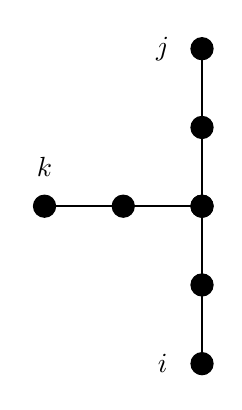
\begin{tikzpicture}
%
\draw[fill=black] (2,2) circle (4pt);
\draw[fill=black] (2,3) circle (4pt);
\draw[fill=black] (2,4) circle (4pt);
\draw[fill=black] (2,1) circle (4pt);
\draw[fill=black] (2,0) circle (4pt);
\draw[fill=black] (0,2) circle (4pt);
\draw[fill=black] (1,2) circle (4pt);
\draw[fill=black] (2,2) circle (4pt);

%
\node at (1.5,0) {$i$};
\node at (1.5,4) {$j$};
\node at (0,2.5) {$k$};
%
\draw[thick] (2,0) -- (2,4);
\draw[thick] (0,2) -- (2,2);

\end{tikzpicture}

%
\begin{caption}[1]
A $3$-armed star with arms of length $2$.
We will eventually use arms of length $t \approx \log n$.
\end{caption}
\label{fig:star}
\end{figure}


The next two lemmas check the conditions to apply Lemma~\ref{lem:basis-conditions} to the sets $\{G^\alpha\}_{\alpha \in \star_\ell(i,j,k)}$.
\begin{lemma}[Unbiased Estimator]\label{lem:block-model-unbiased-estimator}
  Let $i,j,k \in [n]$ all be distinct.
  Let $\alpha \in \star_\ell(i,j,k)$.

  For a collection of probability vectors $\sigma_1,\ldots,\sigma_k$, let $V(\sigma) = \sum_{s \in [k]} v_s^{\tensor 3}$ where $v_s(i) = \sigma_i(s) - \tfrac 1k$.
  Let $G \sim G(n,d,\e,\alpha_0,k)$.
  \[
    \E \Brac{G^\alpha \mid \sigma_i, \sigma_j, \sigma_k } = \Paren{\frac{\e d}{n}}^{3\ell} \Paren{\frac 1 {k(\alpha_0+1)}}^{3(\ell-1)} \cdot C_3 \cdot V(\sigma)_{ijk}\mper
  \]
  Here $\alpha_0 \geq 0$ is the Dirichlet concentration paramter, unrelated to the graph $\alpha$, and $C_3 = 1/(k^{O(1)} \alpha_0^{O(1)})$ is a constant related to third moments of the Dirichlet distribution.
\end{lemma}

\begin{lemma}[Approximate conditional independence]\label{lem:block-model-cond-indep}
If
  \[
  \delta \defeq 1 - \frac{k^2(\alpha_0 +1)^2}{\e^2 d} > 0 \quad \text{ and } \quad k,\alpha_0  \le n^{o(1)} \text{ and } \epsilon^2 d \le n^{o(1)} \mper
  \]
  and $\ell \geq C \log n / \delta^{O(1)}$ for a large enough constant $C$, then for $G \sim G(n,d,\e,k,\alpha_0)$,
  \[
    \E \Brac{V(\sigma)_{ijk}^2} \cdot \sum_{\alpha,\beta \in \star_\ell(i,j,k)} \E G^\alpha G^\beta \leq 1/\delta^{O(1)}\cdot \sum_{\alpha,\beta \in \star_\ell(i,j,k)} \E \Brac{G^\alpha V(\sigma)_{i,j,k}} \cdot \E \Brac{G^\beta V(\sigma)_{i,j,k}}\mper
  \]
\end{lemma}

Now we can prove Lemma~\ref{lem:mm-estimator}.
\begin{proof}[Proof of Lemma~\ref{lem:mm-estimator}]
As discussed at the beginning of this section, it is enough to find an estimator for the tensor $V(\sigma)$.
  Lemma~\ref{lem:block-model-unbiased-estimator} and Lemma~\ref{lem:block-model-cond-indep} show that Lemma~\ref{lem:basis-conditions} applies to each set of polynomials $\star_{\ell}(i,j,k)$.
  The conclusion is that for every distinct $i,j,k \in [n]$ there is a degree $\log n \poly(1/\delta)$ polynomial $P(G)_{ijk}$ so that
  \[
    \frac{\E P(G)_{ijk} V(\sigma)_{ijk}}{(\E P(G)_{ijk}^2)^{1/2} \cdot (\E V(\sigma)_{ijk}^2)^{1/2} } \geq \Omega(1)\mper
  \]
  One may check that the entries $i,j,k$ for $i,j,k$ all distinct of the tensor $V(\sigma)$ comprise nearly all of its $2$-norm.
  That is,
  \[
    \sum_{i,j,k \text{ distinct}} \E V(\sigma)_{i,j,k}^2 \geq (1 - o(1)) \E \|V(\sigma)\|^2\mper
  \]
  This is sufficient to conclude that the tensor-valued polynomial $P(G)$ whose $(i,j,k)$-th entry is $P_{i,j,k}(G)$ when $i,j,k$ are all distinct and is $0$ otherwise is a good estimator of $V(\sigma)$ (see Fact~\ref{fact:scalar-to-vector}).
  Thus,
  \[
    \frac{\E_{\sigma,G} \iprod{P(G), V(\sigma)}}
    {\Paren{\E_{\sigma,G} \Norm{P(G)}^2}^{1/2}  \cdot
    \Paren{\E_{\sigma,G} \Norm{V(\sigma)}^2}^{1/2}} \geq \Omega(1)\mper\qedhere
  \]
\end{proof}


\subsubsection{Details of unbiased estimator}
We work towards proving Lemma~\ref{lem:block-model-unbiased-estimator}.
We will need to assemble a few facts.
The first will help us control moment tensors of the Dirichlet distribution.
The proof can be found in the appendix.

\begin{fact}[Special case of Fact~\ref{fact:dirichlet-covariance}]
\label{fact:diagonal-moments}
  Let $\sigma$ be distributed according to the $\alpha,k$ Dirichlet distribution.
  Let $\tsigma = \sigma - \tfrac 1 k 1$.
  There are numbers $C_2, C_3$ depending on $\alpha,k$ so that for every $x_1, x_2, x_3$ in $\R^k$ with $\sum_{s \in [k]} x_i(s) = 0$,
  \[
    \E_\sigma \iprod{\tsigma, x_1}\iprod{\tsigma, x_2}   = C_2 \iprod{x_1, x_2}
  \]
  and
  \[
    \E_\sigma \iprod{\tsigma, x_1}\iprod{\tsigma, x_2}\iprod{\tsigma,x_3} = C_3 \sum_{s \in [k]} x_1(s) x_2(s) x_3(s)\mper
  \]
  Furthermore,
  \[
    C_2 = \frac 1 {k(\alpha + 1)} \quad \text{ and } \quad C_3 = \frac 1 {k^{O(1)} \alpha^{O(1)}}\mper
  \]
\end{fact}

Now we can prove Lemma~\ref{lem:block-model-unbiased-estimator}.
\begin{proof}[Proof of Lemma~\ref{lem:block-model-unbiased-estimator}]
  For any collection of $\sigma$'s and $\alpha \in \star_\ell(i,j,k)$,
  \begin{align*}
    \E_{G} \Brac{G^\alpha \mid \sigma} & = \Paren{\frac{\epsilon d}{n}}^{3\ell} \prod_{(a,b) \in \alpha} \iprod{\tsigma_a,\tsigma_b}
  \end{align*}
  Let $a$ be the central vertex of the star $\alpha$.
  Taking expectations over all the vertices in the arms of the star,
  \[
  \E \Brac{G^\alpha \mid \sigma_i, \sigma_j, \sigma_k } = \Paren{\frac{\epsilon d}{n}}^{3\ell} \Paren{\frac 1 {k(\alpha_0 +1)}}^{3(\ell-1)} \E_{\sigma_a} \iprod{\tsigma_i,\tsigma_a} \iprod{\tsigma_j,\tsigma_a} \iprod{\tsigma_k,\tsigma_a}\mper
  \]
  Finally, using the second part of Fact~\ref{fact:diagonal-moments} completes the proof.
\end{proof}

\subsubsection{Details of approximate conditional independence}
We prove Lemma~\ref{lem:block-model-cond-indep}, first gathering some facts.
In the sum $\sum_{\alpha, \beta \in \star_\ell(i,j,k) } G^\alpha G^\beta$, the terms $\alpha, \beta$ which (as graphs) share only the vertices $i,j,k$ will not cause us any trouble, because such $G^\alpha$ and $G^\beta$ are independent conditioned on $\sigma_i, \sigma_j, \sigma_k$.
\begin{fact}\label{fact:mm-indep}
  If $\alpha, \beta \in \star_\ell(i,j,k)$ share only the vertices $i,j,k$, then for any collection $\sigma$ of probability vectors,
  \[
    \E\Brac{ G^\alpha G^\beta  \mid \sigma_i, \sigma_j, \sigma_k} = \E \Brac{ G^\alpha \mid \sigma_i, \sigma_j, \sigma_k} \cdot \E \Brac{ G^\beta \mid \sigma_i, \sigma_j, \sigma_k}\mper
  \]
\end{fact}
\begin{proof}
  To sample $G^\alpha$, one needs to know $\sigma_a$ for any $a \in [n]$ with nonzero degree in $\alpha$, and similar for $b \in [n]$ and $G^\beta$.
  The only overlap is $\sigma_i, \sigma_j, \sigma_k$.
\end{proof}

The next fact is the key one.
Pairs $\alpha, \beta$ which share vertices forming paths originating at $i,j,$ and $k$ make the next-largest contribution (after $\alpha, \beta$ sharing only $i,j,k$) to $\sum_{\alpha, \beta} \E G^\alpha G^\beta$.
\begin{fact}\label{fact:mm-path-intersection}
  Let $i,j,k \in [n]$ be distinct.
  Let $V(\sigma)_{ijk}$ be as in the Lemma~\ref{lem:block-model-cond-indep}.
  Let $C_2 \in \R$ be as in Fact~\ref{fact:diagonal-moments}.

  Let $\alpha, \beta \in \star_\ell(i,j,k)$ share $s$ vertices (in addition to $i,j,k$) for some $s \leq \tfrac t 2$, and suppose the shared vertices form paths in $\alpha$ and $\beta$ starting at $i, j, $ and $k$.
  Then
  \[
    \E V(\sigma)_{ijk}^2 \cdot \E G^\alpha G^\beta \leq \e^{-2s} \Paren{\frac{ d} n}^{-s} (1 + O(d/n))^{-s} \cdot \Paren{\frac 1 {k(\alpha_0+1)}}^{-2s} \cdot \E\Brac{ G^{\alpha} V(\sigma)_{ijk}} \cdot \E \Brac{G^{\beta} V(\sigma)_{ijk}} \mper
  \]
\end{fact}
\begin{proof}
  Let $\sigma_{\alpha \cap \beta}$ be the $\sigma$'s corresponding to vertices sharerd by $\alpha, \beta$.
  Let $i', j', k'$ be the last shared vertices along the paths beginning at $i,j,k$ respectively.
  We expand $G^\alpha G^\beta$ and use conditional independence of the $G_e$'s given the $\sigma$'s:
  \[
    \E G^\alpha G^\beta = \E_{\sigma_{i', j', k'} }\Brac{ \E \Brac{ (G^{\alpha \cap \beta})^2 \, | \sigma_{i'}, \sigma_{j'}, \sigma_{k'}} \cdot \E \Brac{G^{\alpha \setminus \beta} \mid \sigma_{i'} \sigma_{j'} \sigma_{k'}} \cdot \E \Brac{G^{\beta \setminus \alpha } \mid \sigma_{i'} \sigma_{j'} \sigma_{k'}}} \mper
  \]
  Both $G^{\alpha \setminus \beta}$ and $G^{\beta \setminus \alpha}$ are long-armed stars with terminal vertices $i', j', k'$.
  The arm lengths of $G^{\alpha \setminus \beta}$ total $3\ell - s$.
  By a similar argument to Lemma~\ref{lem:block-model-unbiased-estimator}, $G^{\alpha \setminus \beta}$ is an unbiased estimator of $V(\sigma)_{i'j'k'}$ with
  \[
    \E\Brac{G^{\alpha \setminus \beta} \mid \sigma_{i'}, \sigma_{j'}, \sigma_{k'}}
    = \Paren{\frac {\e d}n}^{3\ell -s} \Paren{\frac 1 {k(\alpha_0 +1)}}^{3(\ell -1) -s} \cdot C_3 \cdot V(\sigma)_{i', j', k'}
  \]
  and the same goes for $G^{\beta \setminus \alpha}$.
  Furthermore,
  \[
    \E \Brac{ (G^{\alpha \cap \beta})^2 \mid \sigma_{i'}, \sigma_{j'}, \sigma_{k'}}
    = \Paren{\frac dn}^{|\alpha \cap \beta|} \E \Brac{\prod_{(a,b) \in \alpha \cap \beta} (1 + \e \iprod{\tsigma_a, \tsigma_b} + O(d/n)) \, \Big{|} \, \sigma_{i'}, \sigma_{j'}, \sigma_{k'}}\mper
  \]
  By our assumption that $\alpha \cap \beta$ consists just of paths, every subset of edges in the graph $\alpha \cap \beta$ contains a vertex of degree $1$.
  Hence, $\E \Brac{ (G^{\alpha \cap \beta})^2 \mid \sigma_{i'}, \sigma_{j'}, \sigma_{k'}} = (1 + O(d/n))^{|\alpha \cap \beta|} (d/n)^{|\alpha \cap \beta|}$.
  Putting these together,
  \[
    \E G^\alpha G^\beta = (1 + O(d/n))^s \e^{6\ell - 2s} \Paren{\frac dn}^{6\ell - s} \Paren{\frac 1 {k(\alpha_0 +1)}}^{6(\ell-1) - 2s} C_3^2 \E V(\sigma)_{ijk}^2
  \]
  At the same time, one may apply Lemma~\ref{lem:block-model-unbiased-estimator} to $\E G^{\alpha} V(\sigma)_{ijk}$ to obtain
  \[
    \E\Brac{ G^{\alpha} V(\sigma)_{ijk}} \cdot \E \Brac{G^{\beta} V(\sigma)_{ijk}}
    = \Paren{\frac {\e d}n}^{6\ell} \Paren{\frac 1 {k(\alpha_0 + 1)}}^{6(\ell-1)} C_3^2 \cdot \Paren{\E_{\sigma_{i},\sigma_{j}, \sigma_{k}} V(\sigma)_{ijk}^2}^2 \mper
  \]
  The lemma follows.
\end{proof}

The last fact will allow us to control $\alpha, \beta$ which intersect in some way other than paths starting at $i,j,k$.
The key idea will be that such pairs $\alpha, \beta$ must share more vertices than they do edges.
\begin{fact}\label{fact:mm-nonpath-intersection}
  Let $i,j,k \in [n]$ be distinct.
  Let $V(\sigma)_{ijk}$ be as in the Lemma~\ref{lem:block-model-cond-indep}.
  Let $C_2 \in \R$ be as in Fact~\ref{fact:diagonal-moments}. $C_2 = \tfrac 1 {k(\alpha_0+1)}$.

  Let $\alpha, \beta \in \star_\ell(i,j,k)$ share $s$ vertices (in addition to $i,j,k$) and $r$ edges.
  Then
  \[
    \E V(\sigma)_{ijk}^2 \cdot \E G^\alpha G^\beta \leq \e^{-2r} \Paren{\frac dn}^{-r} \cdot C_2^{-2s} \cdot k^{O(s-r)} (1+\alpha_0)^{O(s-r)} \cdot \E\Brac{ G^{\alpha} V(\sigma)_{ijk}} \cdot \E \Brac{G^{\beta} V(\sigma)_{ijk}} \mper
  \]
\end{fact}
\begin{proof}
  Expanding as usual,
  \begin{align*}
  \E G^{\alpha} G^{\beta} = \Paren{\frac dn}^{6\ell - r} \E_\sigma \prod_{ab \in \alpha \triangle \beta} \iprod{\tsigma_a,\tsigma_b} \cdot \prod_{ab \in \alpha \cap \beta} (1 + \e \iprod{\tsigma_a,\tsigma_b} + O(d/n))\mper
  \end{align*}
  Any nontrivial edge-induced subgraph of $\alpha \cap \beta$ contains a degree-1 vertex; using this to expand the second product and simplifying with $\E \tsigma_a = 0$, the above is
  \[
    \Paren{\frac dn}^{6\ell - r} \E_\sigma \prod_{ab \in \alpha \triangle \beta} \iprod{\tsigma_a,\tsigma_b} \cdot (1 + O(d/n))^{r}\mper
  \]
  For every degree-2 vertex in $\alpha \triangle \beta$ we can use Fact~\ref{fact:dirichlet-covariance} to take the expectation.
  Each such vertex contributes a factor of $C_2$ and there are at least $3\ell - O(s-r)$ such vertices.
  The remaining expression will be bounded by $1$.
  The fact follows.
\end{proof}

Now we can prove Lemma~\ref{lem:block-model-cond-indep}.
\begin{proof}[Proof of Lemma~\ref{lem:block-model-cond-indep}]
  Let us recall that our goal is to show
  \[
    \E \Brac{V(\sigma)_{ijk}^2} \cdot \sum_{\alpha,\beta \in \star_\ell(i,j,k) } \E G^\alpha G^\beta \leq \delta^{O(1)} \cdot \sum_{\alpha,\beta \in \star_\ell(i,j,k)} \E \Brac{G^\alpha V(\sigma)_{ijk}} \cdot \E \Brac{G^\beta V(\sigma)_{ijk}}
  \]
  where $\delta = 1 - \tfrac{k^2 (\alpha_0 +1)^2}{\e^2 d}$.
  Let $c = \E \Brac{G^\alpha V(\sigma)_{ijk}} \cdot \E \Brac{G^\beta V(\sigma)_{ijk}}$.
  (Notice this number does not depend on $\alpha$ or $\beta$.)
  The right-hand side above simplifies to $|\star_\ell(i,j,k)|^2 \cdot c$.

  On the left-hand side, what is the contribution from $\alpha,\beta$ sharing $s$ vertices?
  First consider what happens with $s \leq t/2$ and the intersecting vertices form paths in $\alpha$ and $\beta$ starting at $i,j,k$.
  Choosing a random pair $\alpha, \beta$ from $\star_\ell(i,j,k)$, the probability that they intersect along paths of length $s_1, s_2, s_3$ starting at $i,j,k$ respectively is at most $n^{-s_1 - s_2 - s_3}$.
  There are at most $(1 + s^2)$ choices for nonnegative integers $s_1,s_2,s_3$ with $s_1 + s_2 + s_3 = s$.
  By Fact~\ref{fact:mm-path-intersection}, such terms therefore contribute at most
  \[
    c \cdot \frac{|\star_\ell(i,j,k)|^2}{n^{-s}} \cdot \Paren{\epsilon \sqrt{\tfrac d n}(1 + O(d/n))}^{-2s} C_2^{-2s} \cdot s^2
    = c \cdot |\star_\ell(i,j,k)|^2 \cdot (\epsilon^2 d C_2^2 (1 + O(d/n)))^{-s} \cdot s^2
  \]
  where $C_2 = \tfrac 1 {k(\alpha_0 +1)}$.
By hypothesis, $\delta > 0$.
  Consider the sum of all such contributions for $s \leq t/2$; this is at most
  \[
    c \cdot |\star_\ell(i,j,k)|^2 \cdot \sum_{s = 0}^{t/2} (1 + s^2) \cdot \Paren{\tfrac{k^2(\alpha_0+1)^2}{\e^2 d}}^{s} \leq \delta^{O(1)} \cdot c \cdot |\star_\ell(i,j,k)|^2 \mper
  \]

  Next, consider the contribution from $\alpha, \beta$ which share $s$ vertices in some pattern other than those considered above.
  Unless $\alpha = \beta$, this means $\alpha, \beta$ share at least one more vertex than the number $r$ of edges that they share.
  Suppose $\alpha \neq \beta$ and let $s - r = q$.
  There are $t^{O(q)}$ patterns in which such an intersection might occur, and each occurs for a random pair $\alpha, \beta \in \star_\ell(i,j,k)$ with probabilty $n^{-s}$.
  So using Fact~\ref{fact:mm-nonpath-intersection}, the contribution is at most
  \[
    c \cdot |\star_\ell(i,j,k)|^2 \cdot \sum_{q = 1}^{t} \Paren{\frac{\epsilon^2 d}{n}}^q \cdot k^{O(q)} (1+\alpha_0)^{O(q)} t^{O(q)}
  \]
By the hypotheses $k, \alpha = n^{o(1)}$ and $\epsilon^2 d = n^{1 - \Omega(1)}$, this is all $o(c |\star_\ell(i,j,k)|^2)$.

  Finally, consider the case $\alpha = \beta$.
  Then, using Fact~\ref{fact:mm-nonpath-intersection} again, the contribution is at most
  \[
    c \cdot |\star_\ell(i,j,k)|^2 \Paren{\frac{\epsilon^2 d}{k^2 (\alpha_0 + 1)^2}}^{-t} k^{O(1)} \alpha^{O(1)}
  \]
  which is $o(c |\star_\ell(i,j,k)|^2)$ because $t \gg \log(n)$.
  Putting these things together gives the lemma.
\end{proof}

\subsection{Cross validation}
\Snote{}
In this section we show how to use a holdout set of vertices to cross-validate candidate community membership vectors.
The arguments are all standard, using straightforward concentration inequalities.
At the end we prove the first part of Lemma~\ref{lem:xvalid-est}, on the estimator $S_3$.
The proof of the second part, on $S_4$ is similar, using standard facts about moments of the Dirichlet distribution (see Fact~\ref{fact:dirichlet-covariance}).
The proof of Lemma~\ref{lem:xvalid-est-orth} is also similar, using the discussion in Section~\ref{sec:estimator-third-moment} to turn estimators for moments of the $v$ vectors into estimators for moments of the $w$ vectors---we leave it to the reader.

We will need a few facts to prove the lemma.
\begin{fact}
  \label{fact:xvalid-1}
  Let $n_0,n_1,A,k,d,\e,\alpha,\sigma,v,\tau,G,x,P$ be as  in Lemma~\ref{lem:xvalid-est}.
  Let $a \in A$.
  There is a number $C = C(k,\alpha) \leq \poly(k,\alpha)$ such that
  \begin{align*}
  \E_{G,\tau} P_a(G,x)  = \Paren{ \frac{\e d}{n}}^3 \cdot C \cdot \sum_{ijk \in \overline{A} \text{ distinct}} \sum_{s \in [k]} \sigma_i(s) \sigma_j(s) \sigma_k(s) x_i x_j x_k\mper
  \end{align*}
\end{fact}
\begin{proof}
  Immediate from Fact~\ref{fact:diagonal-moments}.
\end{proof}

\begin{fact}
  \label{fact:xvalid-2}
  Let $n_0,n_1,A,k,d,\e,\alpha,\sigma,v,\tau,G,x,P$ be as  in Lemma~\ref{lem:xvalid-est}.
  Let $a \in A$.
  The following variance bound holds.
  \[
    \E_{G,\tau} P_a(G,x)^2 - \Paren{\E_{G,\tau} P_a(G,x)}^2 \leq \frac{\poly(k,\alpha,\e,d)}{n^{3}}\mper
  \]
\end{fact}
\begin{proof}
  Expanding $P_a(G,x)$ and using that $|\iprod{\sigma,\sigma'}| \leq 1$ for any $\sigma, \sigma' \in \Delta_{k-1}$ we get
  \[
    \E_{G,\tau} P_a(G,x)^2  \leq \Paren{\frac{d}{n}}^6 \sum_{\substack{ijk \text{ distinct}\\{i'j'k' \text{ distinct}}}} \Abs{x_i x_j x_k x_{i'} x_{j'} x_{k'} } \leq \Paren{\frac{d}{n}}^6 \cdot n^3 \cdot \|x\|^{12}\mper
  \]
\end{proof}

\begin{fact}
  \label{fact:xvalid-3}
  Let $n_0,n_1,A,k,d,\e,\alpha,\sigma,v,\tau,G,x,P$ be as  in Lemma~\ref{lem:xvalid-est}.
  Let $a \in A$.
  For some constant $\gamma_*(\e,d,k,\alpha)$ and every $\gamma_* > \gamma > 0$,
  \[
    \Pr_{G,\tau} \left \{ |P_a(G,x)| > n^{\gamma} \right \} \leq \exp(-n^{\Omega(\gamma)})
  \]
\end{fact}
\begin{proof}
  The fact follows from a standard exponential tail bound on the degree of vertex $a$.
\end{proof}

We can put these facts together to prove the $S_3$ portion of Lemma~\ref{lem:xvalid-est} (as we discussed above, the $S_4$ portion and Lemma~\ref{lem:xvalid-est-orth} are similar).
The strategy will be to use the following version of Bernstein's inequality, applied to the random variables $\iprod{G_a, v^{\tensor 3}}$.
The proof of the inequality is in the appendix.
\begin{proposition}[Bernstein wth tails]\label{prop:bernstein-tails}
  Let $X$ be a random variable satisfying $\E X = 0$ and, for some numbers $R,\delta,\delta' \in \R$,
  \[
    \Pr \{ |X| > R \} \leq \delta \text{ and } \E|X|\cdot \Ind_{|X| > R} \leq \delta'\mper
  \]
  Let $X_1,\ldots,X_m$ be independent realizations of $X$.
  Then
  \[
    \Pr \left \{ \Abs{\tfrac 1 m \sum_{i \leq m} X_i} \geq t + \delta' \right \} \leq \exp\Paren{\frac{- \Omega(1) \cdot m \cdot t^2}{\E X^2 + t\cdot R}} + m \delta \mper
  \]
\end{proposition}

Now we can prove Lemma~\ref{lem:xvalid-est}.

\begin{proof}[Proof of Lemma~\ref{lem:xvalid-est}]
  We apply Proposition~\ref{prop:bernstein-tails} to the $n_1$ random variables $X_a = \Paren{\tfrac{\e d} n}^{-3} C^{-1} P_a(G,x)$ for $a \in A$, where $C = C(k,\alpha)$ is the number from Fact~\ref{fact:xvalid-2}.
  (For each $a \in A$ these are iid over $G,\tau$.)
  Take $t = n^{3/2 - \gamma'}$ for a small-enough constant $\gamma'$ so that $n_1t^2/n^3 \geq n^{\gamma}$ for some constant $\gamma$, using the assumption $n_1 \geq n^{\Omega(1)}$.
  All together, we get
  \[
  \Pr_{G,\tau} \left \{ \Abs{\frac 1 {n_1} \sum_{a \in A} X_a - \sum_{s \in [k]} \sum_{ijk \in \overline A \text{ distinct}} \sigma_s(i) \sigma_s(j) \sigma_s(k) x_i x_j x_k } \geq n^{3/2 - \gamma'} \right \} \leq \exp(n^{-\gamma'})
  \]
  for some constants $\gamma, \gamma'$ (possibly different from $\gamma, \gamma'$ above) and large-enough $n$.
  For any unit $x \in \R^{n_0}$ and $\sigma \in \Delta_{k-1}^{n_0}$, using that $k \leq n^{o(1)}$ it is not hard to show via Cauchy-Schwarz that
  \[
  \Abs{\sum_{s \in [k]} \iprod{v_s,x}^3 - \sum_{s \in [k]} \sum_{ijk \in \overline A \text{ distinct}} \sigma_s(i) \sigma_s(j) \sigma_s(k) x_i x_j x_k} \leq n^{1 + o(1)}\mper
  \]
  The lemma follows.
\end{proof}

\subsection{Producing probability vectors}
\newcommand{\ov}{\overline{v}}
\newcommand{\ow}{\overline{w}}

In this section we prove Lemma~\ref{lem:cleanup}.
The proof of Lemma~\ref{lem:cleanup-2} is very similar (in fact it is somewhat easier) so we leave it to the reader.
\restatelemma{lem:cleanup}
 First some preliminaries.
Let $\sigma_1,\ldots,\sigma_n$ be iid from the $\alpha,k$ Dirichlet distribution.
There are two important families of vectors in $\R^n$.
Let
\[
v_s(i) = \sigma_i(s) - \frac 1k \qquad w_s(i) = \sigma_i(s) - \frac 1k\Paren{1 - \frac 1 {\sqrt{\alpha+1}}}\mper
\]
We will also work with a normalized version of the $v$ vectors:
\[
  \overline{v}_s = \frac{v_s}{(\E\|v_s\|^2)^{1/2}}\mper
\]
By construction, $\E\|\overline{v}_s\|^2 = 1$.
Also by definition, $\sum_s v_s = \sum_s \overline{v}_s = 0$.
Thus $\E \iprod{\sum_s \ov_s ,\sum_s \ov_s} = k + \sum_{s \neq t} \E\iprod{\ov_s,\ov_t} = 0$ and so by symmetry $\E \iprod{\ov_s,\ov_t} = \frac{-1}{k-1}$.
We let
\[
\ow_s = \ov_s + \frac 1{\sqrt n} \cdot \sqrt{\frac 1 {k-1}}
\]
so that $\E \iprod{\ow_s,\ow_t} = 0$ for $s \neq t$.
(In the facts which follow we sometimes write $\ov$ as $v$ when both normalizations are not needed; this is always noted.)

We will want the following fact; the proof is elementary.
\begin{fact}\label{fact:v-corr}
  Let $\sigma,u,v,w$ as above, and suppose $y$ is an $n \times k$ matrix whose rows are in $\Delta_{k-1} - \tfrac 1k$ (that is they are shifted probability vectors).
  Then $\tau = y + \tfrac 1k$ is a matrix whose rows are probability vectors, and $\tau$ satisfies
  \[
    \iprod{\tau,\sigma} \geq \iprod{y,v} + \frac nk\mper
  \]
\end{fact}

The following fact will be useful when $\delta$ is small but not tiny; i.e. $\delta < 1 - c$ for some fixed constant $c$ but $\delta \gg 1/\sqrt k$.
\begin{fact}
\label{fact:permutation-small}
  Suppose that $x_1,\ldots,x_k$ are unit vectors and $w_1,\ldots,w_k$ are orthonormal.
  Also suppose that there is $1 > \delta > 0$ such that for at least $\delta k$ vectors $w_s$ among $w_1,\ldots,w_k$ there exists a vector $x_t$ among $x_1,\ldots,x_k$ such that $\iprod{w_s,x_t} \geq \delta$.
  Then there is a permutation $\pi : [k] \rightarrow [k]$ such that if $x = (x_1,\ldots,x_k)$ is an $n \times k$ matrix and similarly for $w$,
  \[
  \iprod{x, \pi \cdot w} \geq \Paren{\delta^5 - \frac 1 {\sqrt k}\Paren{\frac 1 {1-\delta^4}}^{1/2}} \|x\|\|w\|\mcom
  \]
  where $x = (x_1,\ldots,x_k)$ is an $n \times k$ matrix and similarly for $w$.
\end{fact}
\begin{proof}
  We will think of $\pi$ as a matching of $w_1,\ldots,w_k$ to $x_1,\ldots,x_k$.
  Call $x_t$ \emph{good} for $w_s$ if $\iprod{w_s,x_t} \geq \delta$.
  First of all, by orthogonality of vectors $w_1,\ldots,w_k$, any particular vector $x_t$ is good for at most $1/\delta^2$ vectors $w_s$.
  Hence, there is a set $S$ of $\delta^4 k$ vectors $w_s$ such that for each $w_s$ there exists a good $x_t$ and all the good $x_t$'s are distinct.

  Begin by matching each $w_s \in S$ to its good $x_t$.
  Let $\pi$ be the result of extending that matching randomly to a perfect matching of $k$ to $k$.

  We need to lower bound $\E \sum_{s \notin S} \iprod{w_s,x_{\pi (s)}}$.
  Consider that for a particular $t$,
  \[
  \E -\iprod{x_t, w_{\pi^{-1}(t)}} \leq (\E \iprod{x_t, w_{\pi^{-1}(t)}}^2)^{1/2}\mper
  \]
  The distribution of $\pi^{-1}(t)$ is uniform among all $s \notin S$.
  So
  \[
    \E \iprod{x_t, w_{\pi^{-1}(t)}}^2 = \frac 1 {k - |S|} \sum_{s \notin S} \iprod{w_s,x_t}^2 \leq \frac 1k \Paren{\frac 1 {1 - \delta^4}}
  \]
  since $\sum_{s \in [k]} \iprod{w_s,x_t}^2 \leq 1$.
  It follows that
  \[
    \E \iprod{x_t, w_{\pi^{-1}(t)}} \geq - \frac 1 {\sqrt k} \Paren{\frac 1 {1-\delta^4}}^{1/2}\mper
  \]
  Therefore, $\E \sum_{s \notin S} \iprod{w_s, x_{\pi(s)}} \geq - \sqrt k\Paren{\frac 1 {1-\delta^4}}^{1/2}$.
  Thus there is some choice of $\pi$ such that $\sum_{s \notin S} \iprod{w_s, x_{\pi(s)}} \geq - \sqrt k\Paren{\frac 1 {1-\delta^4}}^{1/2}$.
  Hence for this $\pi$ one gets
  \[
    \sum_{s \in [k]} \iprod{w_s,x_{\pi(s)}} \geq \delta^5 k - \sqrt k\Paren{\frac 1 {1-\delta^4}}^{1/2} = \Paren{\delta^5 - \frac 1 {\sqrt k}\Paren{\frac 1 {1-\delta^4}}^{1/2}} \|x\|\|w\|\mper\qedhere
  \]
\end{proof}

The next fact serves the same purpose as the previous one but in the large $\delta$ case (i.e. $\delta$ close to $1$).
\begin{fact}
\label{fact:permutation-large}
  Under the same hypotheses as Fact~\ref{fact:permutation-small}, letting $\delta = 1 - \e$ for some $\e > 0$, there is a permutation $\pi : [k]  \rightarrow [k]$ such that $\iprod{x,\pi \cdot w} \geq (1 - 9\e) \|x\|\|w\|$.
\end{fact}
\begin{proof}
  As in the proof of Fact~\ref{fact:permutation-small}, we construct a matching $\pi$ by first matching a set $S$ of at least $\delta^4k \geq (1 - 4\e)k$ vectors $w_s$ to corresponding $x_t$.
  Then we match the remaining vectors arbitrarily.
  For any $s,t$ we know $\iprod{w_s,x_t} \geq -1$.
  So the result is
  \[
  \iprod{x, \pi \cdot w} \geq (1 - 5 \e) k - 4 \e k = (1 - 9 \e) k = (1 - 9\e) \|x\|\|w\|\mper\qedhere
  \]
\end{proof}

We will also want a way to translate a matrix correlated with $w$ to one correlated with $v$, so that we can apply Fact~\ref{fact:v-corr}.
\begin{fact}
  \label{fact:shift-1}
  Suppose $v$ is an $n \times k$ matrix whose rows are centered probability vectors and $w = v + c$ is a coordinate-wise additive shift of $v$.
  Suppose $y$ is also an $n \times k$ matrix whose rows are centered probability vectors shifted by $c$ in each coordinate (so $y - c$ is a matrix of centered probability vectors).
  Then the shifted matrix $y-c$ satisfies
  \[
    \iprod{y-c,v} \geq \iprod{y,w} - c^2 nk\mper
  \]
\end{fact}
\begin{proof}
  By definition, $\iprod{y -c,v} = \iprod{y,v}$. Since $v = w -c$, we get
  \[
    \iprod{y-c,v} = \iprod{y,v} = \iprod{y,w} - c \iprod{y, 1} = \iprod{y,w} - c^2 nk\mper\qedhere
  \]
\end{proof}

\begin{proof}[Proof of Lemma~\ref{lem:cleanup}]
  First assume $\delta < 1 - c$ for any small constant $c$.
  Let $\pi$ be the permutation guaranteed by Fact~\ref{fact:permutation-small} applied to the vectors $x_1,\ldots,x_k$ and $M^{-1/2}w_1,\ldots,M^{-1/2}w_k$.
  (Without loss of generality reorder the vectors so that $\pi$ is the identity permutation.)
  Since $1-c \geq \delta \geq 1/k^{1/C}$ for big-enough $C$ and small-enough $c$ (which are independent of $n,k$) and the guarantee of Fact~\ref{fact:permutation-small}, by event $E$ we get that
  \[
    \iprod{x,w} \geq \delta^{O(1)} \|x\| \|w\|\mper
  \]
  So by taking a correlation-preserving projection of $x$ into the set of matrices whose rows are shifted probability vectors, we get a matrix $y$ with the guarantee
  \[
  \iprod{y,w} \geq \delta^{O(1)} \|y\| \|w\| \quad \text{ and } \quad \|y\| \geq \delta^{O(1)} \|w\|\mper
  \]
  Applying Fact~\ref{fact:shift-1}, we obtain
  \[
  \iprod{y -c,v} \geq \iprod{y,w} - c^2 nk = \iprod{y,w} - \frac{\E \|w\|^2}{k}
  \]
  where $c = \tfrac 1 {k \sqrt{\alpha+1}}$.
  Putting things together and using $\E \|v\|^2 \leq \E \|w\|^2$ and the event $E$, we get
  \[
    \iprod{y-c,v} \geq \delta^{O(1)} \E\|v\|^2\mper
  \]
  So applying Fact~\ref{fact:v-corr} finishes the proof in this case.

  Now suppose $\delta \geq 1 -c$ for a small-enough constant $c$.
  Then using event $E$ and Fact~\ref{fact:permutation-large}, there is $\pi$ such that $\iprod{x,w} \geq (1 - O(c)) \|x\|( \E \|w\|^2)$ (where again we have without loss of generality reordered the vectors so that $\pi$ is the identity permutation).
 Now taking the Euclidean projection of $x \cdot \frac{(\E \|w\|^2)^{1/2}}{\|x\|}$ into the $n \times k$ matrices whose rows are centered probability vectors shifted entrywise by $c = \tfrac 1 {k\sqrt{\alpha+1}}$, we get a matrix $y$ which again satisfies
 $\iprod{y,w} \geq (1 - O(c)) \|y\|\|w\|$ and $\|y\| \geq (1 - O(c)) \|w\|$, so (using event $E$), $\iprod{y,w} \geq (1 - O(c)) \E \|w\|^2$.
 Removing the contribution from $\iprod{y,1}$, this implies that $\iprod{y-c,v} \geq (1 - O(c)) \E \|v\|^2$.
 For $c$ small enough, this is at least $\delta^{O(1)} \E \|v\|^2$.
 Applying Fact~\ref{fact:v-corr} finishes the proof.
\end{proof}


\subsection{Remaining lemmas}
We provide sketches of the proofs of Lemma~\ref{lem:shift-and-whiten} and Lemma~\ref{lem:cleanup}, since the proofs of these lemmas use only standard techniques.

\begin{proof}[Proof sketch of Lemma~\ref{lem:shift-and-whiten}]
  For $\sigma \in \R^k$, let $\tilde{\sigma} = \sigma - (1 - 1/\sqrt{\alpha+1})/k$.
  Standard calculations show that if $\sigma$ is drawn from the $\alpha,k$ Dirichlet distribution then $\E \tsigma \tsigma^\top = \tfrac 1 {k(\alpha+1)} \Id$.
  It follows by standard matrix concentration and the assumption $k,\alpha \leq n^{o(1)}$ that the eigenvalues of $\frac 1n \sum_{i \leq n} \tsigma_i \tsigma_i^\top$ are all $1 \pm n^{-\Omega(1)}$, where $\sigma_1,\ldots,\sigma_n$ are iid draws from the $\alpha,k$ Dirichlet distribution.

  For the second part of the Lemma, use the first part to show that $\Norm{\tfrac{v_s}{\|v_s\|} - w'_s} \leq 1/\poly(k)$.
  Then when $k \geq \delta^{-C}$ for large-enough $C$, if $\iprod{x,v_s}^3 \geq \delta^{O(1)} \|v_s\|^3$ it follows that also $\iprod{x,w_s} \geq \delta^{O(1)} - 1/\poly(k) \geq \delta^{O(1)}$.
  The lemma follows.
\end{proof}

\begin{proof}[Proof sketch of Lemma~\ref{lem:cleanup}]
  If $\delta < 1 - \Omega(1)$, then $\delta^2/2 \geq \delta^{O(1)}$, so the Lemma follows from standard concentration and Theorem~\ref{thm:correlation-preserving-projection} on correlation-preserving projection.
  On the other hand, if $\delta \geq 1 - o(1)$, then $\|v' - \tsigma\| \leq o(1) \cdot \|\tsigma\|$, so the same is also true for the projection of $v'$ into $(\tilde{\Delta}_{k-1})^n$ by convexity and the lemma follows.
\end{proof}




\iffalse


We work with very sparse graphs---essentially they are samples from $G(n,d,\e, \alpha,k)$ where $\epsilon^2 d > \eta \cdot k^2 (\alpha + 1)^2$ for some constant $\eta > 0$.
(This is as opposed to the setting for recovery, when $\epsilon^2 d > (1 + \Omega(1)) k^2 (1 + \alpha)$.)
To ensure that we are using fresh randomness in the cross validation we have to condition on the partition $H_1, H_2$.
This means the graph we use in this step will not exactly have the block model distribution, but the estimation facts we need will still hold.

Our main tool to prove Lemma~\ref{lem:xvalid-main} will be the following.



\begin{lemma}\label{lem:xvalid-main-estimator}
  Let $G$ be the holdout graph as in the partial recovery algorithm, with expected average degree $h$.
  Suppose $\epsilon^2 h > \eta k^2 (k\alpha + 1)^2$ for some $\eta = \Omega(1)$.
  Suppose $k, \alpha, \epsilon^2 h \leq n^{o(1)}$

  Let $A, \overline A$ be a random patition of $[n]$ into two sets of size $\tfrac n 2$.
  Let $v_s \in \R^{\overline A}$ for $s \in [k]$ be the vectors $v_s(i) = \sigma_i(s) - \tfrac 1 k$ for $i \in \overline A$.
  Let $v \in \R^{\overline A}$ be a unit vector with $|v(i)| \leq n^{-1/2 + o(1)}$ for each coordinate $i \in \overline A$.

  For $a \in A$, let $H_a$ be the $3$-tensor indexed by $i,j,k \in \overline A$ with $(H_a)_{i,j,k} = H_{ai}H_{aj}H_{ak}$ when $i,j,k$ are all distinct and the pairs $(i,a), (j,a), (k,a)$ all belong to $H_2$, and $0$ otherwise.
  Here $H_{ab}$ is the centered indicator $H_{ab} = x_{ab} - \tfrac dn$.

  There is a number $c$ so that with probability at least $1-n^{-\omega(1)}$, conditioned on $H_1$ and $H_2$,
  \[
    \Abs{\frac 1 {c |A|} \sum_{a \in A} \iprod{H_a, v^{\tensor 3}} - \sum_{s \in [k]} \iprod{v_s, v}^3} \leq n^{3/2 - \Omega(1)}\mper
  \]
\end{lemma}

From this we can prove Lemma~\ref{lem:xvalid-main}

\begin{proof}[Proof of Lemma~\ref{lem:xvalid-main}]
  First suppose that the unit vector $x$ has some coordinates with $|x(i)| > n^{-1/2 + \Omega(1)}$.
  Let $S \subseteq [n]$ be the set of such coordinates.
  Since $x$ is a unit vector, there can only be $n^{1-\Omega(1)}$ such coordinates.
  The vectors $v_s$ all have (with high probability) all coordinates bounded by $n^{-1/2 + o(1)}$ in magnitude.
  So, for any $v_s$,
  \[
    \Abs{\sum_{i \in [S]} v_s(i) x(i) } \leq \Paren{\sum_{i \in S} v_s(i)^2}^{1/2} \leq n^{-\Omega(1)}
  \]
  Setting all such coordinates of $x$ to zero affects $\iprod{x,v_s}$ be only $n^{-\Omega(1)}$ additively, so we assume $x$ has all coordinates at most $n^{-1/2 + o(1)}$ in magnitude.

  The oracle computes the value of the estimator from Lemma~\ref{lem:xvalid-main-estimator}, obtaining a number
  \[
    a = \frac 1 {(\E \|v_s\|^2)^{3/2}} \sum_{s \in [k]} \iprod{v_s,x}^3 \pm n^{-\Omega(1)}\mper
  \]
  The norms $\|v_s\|^2$ are highly concentrated (this can be proved via standard techniques).
  The lemma follows.
\end{proof}


For the remainder of the section we turn to proving Lemma~\ref{lem:xvalid-main-estimator}.
The proof will re-use many of the ideas from previous sections.
First, we show that the $G_a$'s are unbiased estimators of (the multilinear part of) $\sum_{s \in [k]} v_s^{\tensor 3}$.

\begin{lemma}\label{lem:xvalid-unbiased-estimator}
  Consider the same setup as in Lemma~\ref{lem:xvalid-main-estimator}.
  Let
  \[
    f(v) = \sum_{s \in [k]} \sum_{i,j,k \in \overline A \text{ all distinct}} v(i) v(j) v(k) v_s(i) v_s(j) v_s(k)
  \]
  be the multilinear part of the polynomial $\sum_{s \in [k]} \iprod{v_s,v}^3$.
  Let $\sigma_{\overline A}$ be the subset of $\sigma_i$'s corresponding to $i \in \overline A$.
  For every $a \in A$ and $\sigma$,
  \[
    \E_G\Brac{ \iprod{H_a, v^{\tensor 3}} \mid A,\sigma_{\overline A}} = \Paren{\frac {\e h} n}^3 \cdot k^{-O(1)} \alpha^{-O(1)} \cdot  f(v)
  \]
\end{lemma}
\begin{proof}
  We expand the above expression
  \begin{align*}
    \E_G & \Brac{  \iprod{G_a, v^{\tensor 3}} \mid A,\sigma_{\overline A}}\\
    & = \Paren{\frac{\e h} n}^{3} \E_{\sigma_a} \sum_{i,j,k \in \overline A \text{ histinct}} \iprod{\sigma_a,\sigma_i}\iprod{\sigma_a,\sigma_j}\iprod{\sigma_a,\sigma_k} \cdot v(i) v(j) v(k)\\
    & = \Paren{\frac{\e h} n}^{3} \cdot C_3 \cdot \sum_{i,j,k \in \overline A \text{ distinct}} \sum_{s \in [k]} v_s(i) v_s(j) v_s(k) v(i) v(j) v(k) \text{ for $C$ as in Fact~\ref{fact:diagonal-moments}}\\
    & = \Paren{\frac {\e h} n}^{3} \cdot k^{-O(1)} \alpha^{-O(1)} \cdot f(v)\mper\qedhere
  \end{align*}
\end{proof}

We will also need to control the variance of each $\iprod{G_a, v^{\tensor 3}}$.
\begin{lemma}\label{lem:xvalid-Ha-variance}
  With the same notation as in Lemma~\ref{lem:xvalid-unbiased-estimator},
  $ \Var[ \iprod{H_a, v^{\tensor 3}} \mid A, \sigma_{\overline A} ]  \leq O(n^{-3} \epsilon^2 h)^6$.
\end{lemma}
\begin{proof}
  We expand the second moment, which bounds the variance.
  \begin{align*}
    \E_{H | \sigma_{\overline A}} \iprod{H_\alpha, v^{\tensor 3}}^2
    & = \sum_{
      \substack{i,j,k \in \overline A \text{ distinct}\\
        i',j',k' \in \overline A \text{ distinct}}}
      v(i) v(j) v(k) v(i') v(j') v(k') \E_{H | \sigma} H_{ai} H_{aj} H_{ak} H_{ai'} H_{aj'} H_{ak'} \\
      & \leq \Paren{\sum_{
      \substack{i,j,k \in \overline A \text{ distinct}\\
        i',j',k' \in \overline A \text{ distinct}}} [v(i) v(j) v(k) v(i') v(j') v(k')]^2}^{1/2} \\
      & \cdot \Paren{\sum_{
      \substack{i,j,k \in \overline A \text{ distinct}\\
        i',j',k' \in \overline A \text{ distinct}}}
      (\E_{H | \sigma} H_{ai} H_{aj} H_{ak} H_{ai'} H_{aj'} H_{ak'})^2 }^{1/2}\mper
  \end{align*}

  The first term is at most $\|v\|^{O(1)} = 1$.
  As for the second term,
  when all $i,j,k,i',j',k'$ are distinct,
  \begin{align*}
    (\E_{H | \sigma_{\overline A}} & H_{ai} H_{aj} H_{ak} H_{ai'} H_{aj'} H_{ak'})^2\\
    & = \Paren{\frac{\e h} n}^{12} \cdot (\E \iprod{\tsigma_a,\tsigma_i}\iprod{\tsigma_a,\tsigma_j}\iprod{\tsigma_a,\tsigma_k}\iprod{\tsigma_a,\tsigma_{i'}}\iprod{\tsigma_a,\tsigma_{j'}}\iprod{\tsigma_a,\tsigma_{k'}})^2 \\
    & \leq \Paren{\frac{\e h}n}^{12}
  \end{align*}
  So the contribution from $i,j,k,i',j',k'$ all distinct is at most
  \[
    \Paren{n^6 \cdot \Paren{\frac{\e h} n}^{12}}^{1/2} \leq O(n^{-3} \epsilon^2 h)^{6}\mper
  \]
  Similar computations apply to handle the cases that $i,j,k,i',j',k'$ are not all distinct.
\end{proof}

The last thing we will need to apply Bernstein's inequality is a bound of the form $\Pr \{ | \iprod{H_a, v^{\tensor 3}} | > R \mid A, \sigma_{\overline A} \} \leq \delta$.
This will use our assumption that the entries of $v$ are not too big.

\begin{lemma}\label{lem:xvalid-truncation}
  Consider the same setup as in Lemma~\ref{lem:xvalid-main-estimator},
  \[
    \Pr \{ | \iprod{H_a, v^{\tensor 3}} | > n^{-3/2 + o(1)} \mid A, \sigma_{\overline A}  \} \leq n^{-\omega(1)} \mper
  \]
\end{lemma}
\begin{proof}
  Inspecting the expansion of $\iprod{H_a, v^{\tensor 3}}$,
  \[
    \iprod{H_a, v^{\tensor 3}} = \sum_{i,j,k \in \overline{A} \text{ distinct}} H_{ai} H_{aj} H_{ak} v_i v_j v_k\mper
    \]
  Standard concentration shows $a$ has degree that at most $(\log n)^{O(1)}$ with probability $n^{-\omega(1)}$.
  Consider first the triples $i,j,k$ all of which have an edge to $a$.
  When $a$ has degree $(\log n)^{O(1)}$, there are at most $(\log n)^{O(1)}$ such triples, each contributing $H_{ai} H_{aj} H_{ak} = O(1)$.
  Since $|v_i v_j v_k| < n^{-3/2 + o(1)}$, the contribution from the corresponding terms is at most $n^{-3/2 + o(1)}$.
  Similar considerations apply for other kinds of triples.
\end{proof}

Now we can prove Lemma~\ref{lem:xvalid-main-estimator}.
\begin{proof}[Proof of Lemma~\ref{lem:xvalid-main-estimator}]
  Conditioned on $A, \sigma_{\overline A}$, the random variables $\iprod{H_a, v^{\tensor 3}}$ are iid.
  Each has variance $O(n^{-3} \epsilon^2 d)^{6}$ and is at most $n^{-3/2 + o(1)}$ in magnitude with probability $1 - n^{-\omega(1)}$.
  So we can apply Proposition~\ref{prop:bernstein-tails} to obtain that with probability $n^{-\omega(1)}$,
  \[
    \Abs{\frac 1 {|A|} \sum_{a \in A} (\iprod{H_a, v^{\tensor 3}} - \E \iprod{G_a, v^{\tensor 3}})} \leq n^{-3/2 - \Omega(1)}
  \]
  (Here the expectations are conditioned on $A, \sigma_{\overline A}$.)
   So by Lemma~\ref{lem:xvalid-unbiased-estimator}, there is a number $c =  \Paren{\frac {\e h} n}^{3} \cdot k^{-O(1)} \alpha^{-O(1)}$
  so that
  \[
    \Abs{\frac 1 {c \cdot |A|} \sum_{a \in A} \iprod{H_a, v^{\tensor 3}} - f(v)} \leq n^{-3/2 - \Omega(1)} / c = n^{3/2 - \Omega(1)}\mper
  \]
  It just remains to check that $f(v) - \sum_{s \in [k]} \iprod{v_s,v}^3$ is not too large.
  This follows from the assumption that $v$ has no large entries.
  \[
    f(v) - \sum_{s \in [k]} \iprod{v_s,v}^3 = - \sum_{s \in [k]} \sum_{i,j,k \in \overline{A} \text{ not all distinct}} v(i) v(j) v(k) v_s(i) v_s(j) v_s(k)\mper
  \]
  Consider the contribution from a single $s$ and the terms where $i = j$.
  We get
  \[
    \sum_{i,k} v(i)^2 v_s(i)^2 v(k) v_s(k) = \sum_{i} v(i)^2 v_s(i)^2 \cdot \iprod{v,v_s} \leq n^{-1 + o(1)} \cdot \|v_s\|^2 \cdot \iprod{v,v_s} \leq n^{1/2 + o(1)}
  \]
where we have used Cauchy-Schwarz as well as straightforward bounds on $\|v_s\|^2$.
The remaining cases are similar.
\end{proof}

\fi